% =====================================================================
%  Attribution Limits of AI Pentest Agents
%  arXiv submission package.
%
%  Build:  pdflatex main && bibtex main && pdflatex main && pdflatex main
%  Everything needed is inside this directory (figures/ is copied here).
% =====================================================================
\documentclass[11pt]{article}

% --- encoding / fonts (all standard TeX Live, all available on arXiv) ---
\usepackage[T1]{fontenc}
\usepackage[utf8]{inputenc}
\usepackage{lmodern}

% --- page geometry ---
\usepackage[margin=1in]{geometry}

% --- graphics / maths ---
\usepackage{graphicx}
\usepackage{amsmath}
\usepackage{amssymb}

% --- tables ---
\usepackage{booktabs}
\usepackage{array}
\usepackage{tabularx}
\usepackage{longtable}

% --- code blocks ---
\usepackage{listings}

% --- colour / typography / captions ---
\usepackage{xcolor}
\usepackage{microtype}
\usepackage{caption}

% --- hyperlinks (loaded last) ---
\usepackage[hidelinks,breaklinks]{hyperref}

% ---------------------------------------------------------------------
%  Global table and listing settings
% ---------------------------------------------------------------------
\renewcommand{\arraystretch}{1.15}
\setlength{\tabcolsep}{6pt}
\captionsetup{font=small,labelfont=bf,labelsep=period,skip=4pt}
\setlength{\textfloatsep}{11pt plus 2pt minus 4pt}
\setlength{\floatsep}{9pt plus 2pt minus 3pt}
\setlength{\intextsep}{11pt plus 2pt minus 4pt}
\setlength{\abovecaptionskip}{3pt}
\setlength{\belowcaptionskip}{0pt}

\newcolumntype{Y}{>{\raggedright\arraybackslash}X}
\newcolumntype{L}[1]{>{\raggedright\arraybackslash}p{#1}}
\newcolumntype{R}[1]{>{\raggedleft\arraybackslash}p{#1}}

\lstset{
  basicstyle=\ttfamily\small,
  columns=fullflexible,
  keepspaces=true,
  breaklines=true,
  frame=single,
  framerule=0.4pt,
  xleftmargin=0.4em,
  aboveskip=0.9em,
  belowskip=0.9em,
  showstringspaces=false
}

% ---------------------------------------------------------------------
%  Title block
% ---------------------------------------------------------------------
\title{\textbf{Attribution Limits of AI Pentest Agents}\\
An Empirical Study of 65 Audited Codebases, 272 Validated Traffic
Signatures, and the Boundary Where Attribution Stops Working}

\author{The \texttt{ai-agent-attack-signatures} contributors\\
\small Artefact repository: \url{https://github.com/Raven-Gt/ai-agent-attack-signatures}}

\date{}

\begin{document}

\maketitle
\thispagestyle{plain}

\begin{abstract}
AI-assisted penetration-testing agents are being deployed to automate reconnaissance and
exploitation at scale. The defensive question that follows is whether such traffic can be
identified and attributed on the victim network. This paper reports an empirical study of
65 AI-pentest codebases (64 third-party frameworks plus one in-house implementation),
combining static source auditing with live traffic collection and scoring against three
real-world corpora.

We extract 610 traffic signatures and tier them by attributability: 272 are framework-exclusive
and observable in an HTTP access log (T1), 126 express generic attack semantics (T2), and 212
are generic tooling identifiers or over-broad patterns (T3). The T1 set is validated against
9,905,794 public internet requests from 80,987 source addresses and 142,705 real WAF attack
transactions spanning 30 days; it matches zero rules in both corpora, and exactly one source
address matches two or more rules.

Alongside the signatures we build an actor-level behavioural detector whose decision unit is
the actor (all requests from one source address within a time window). Forty-three features
grouped into ten families feed fourteen evidence rules fused with a noisy-OR model. Across 15
live agent captures covering 12 frameworks the detector reaches 86.7\% segment recall and 83.3\%
framework recall (one-sided 95\% lower bound 0.779), retains 90\% recall under
leave-one-framework-out, and runs at a 2.72\% false-positive rate on 1,582 real attacker actors
(95\% CI [2.02\%, 3.64\%]).

The central negative result is that attribution and detection are different problems, and
neither is solved by signatures alone. An agent that delegates to sqlmap, ffuf or nuclei is
indistinguishable from a human running the same tool: on six scanner actors the false-positive
rate is 66.67\% and raising the decision threshold does not help. We quantify this boundary
with three independent pieces of evidence, and show that the only reliable attribution signal
for an AI agent is its outbound traffic to an LLM gateway, which requires egress logs rather
than passive inspection.

We release the signatures, the captured datasets and the evaluation code so that every
reported measurement can be reproduced and extended.
\end{abstract}

\noindent\textbf{Repository.} This paper is the paper associated with the
\texttt{ai-agent-attack-signatures} repository, which ships the signatures, the captured
datasets and the evaluation code: \url{https://github.com/Raven-Gt/ai-agent-attack-signatures}
\cite{aasrepo}. Every number quoted below is asserted by continuous integration against the
shipped artefacts, and the artefact is self-contained: the LaTeX sources, the compiled PDF and
the twelve vector figures used here all live in the \texttt{paper/} directory of that
repository.

% =====================================================================
\section{Introduction}
\label{sec:intro}

AI pentest agents promise to compress the reconnaissance and exploitation phases of an
assessment into a single supervised loop. They are actively being integrated into CI
pipelines, bug-bounty triage and continuous penetration testing. The defender's question is
concrete: given a stream of HTTP requests to a protected asset, can we tell that they were
produced by an AI agent rather than by a person --- and if so, which agent?

Signature catalogues exist for conventional tooling, and the obvious move is to apply the same
recipe to AI agents: read the source, extract the distinguishing strings, ship the rules. This
paper reports doing exactly that for 65 codebases, and then measuring how far the result
actually gets on real traffic.

Three findings shape the contribution.

\textbf{Finding 1 --- the majority of AI agents leave no framework-specific trace on the
target.} Most frameworks do not issue HTTP requests themselves; they orchestrate external
tools (sqlmap, ffuf, nuclei, nmap, curl) through a shell. The target therefore observes the
tool, not the agent. Of 65 audited codebases, only 10 were validated end-to-end as
attributable on the target side. A signature set built naively from source code would mostly
encode strings that never reach a victim.

% source artwork: figures/fig01_framework_attribution_matrix.pdf
\begin{figure}[t]
\centering
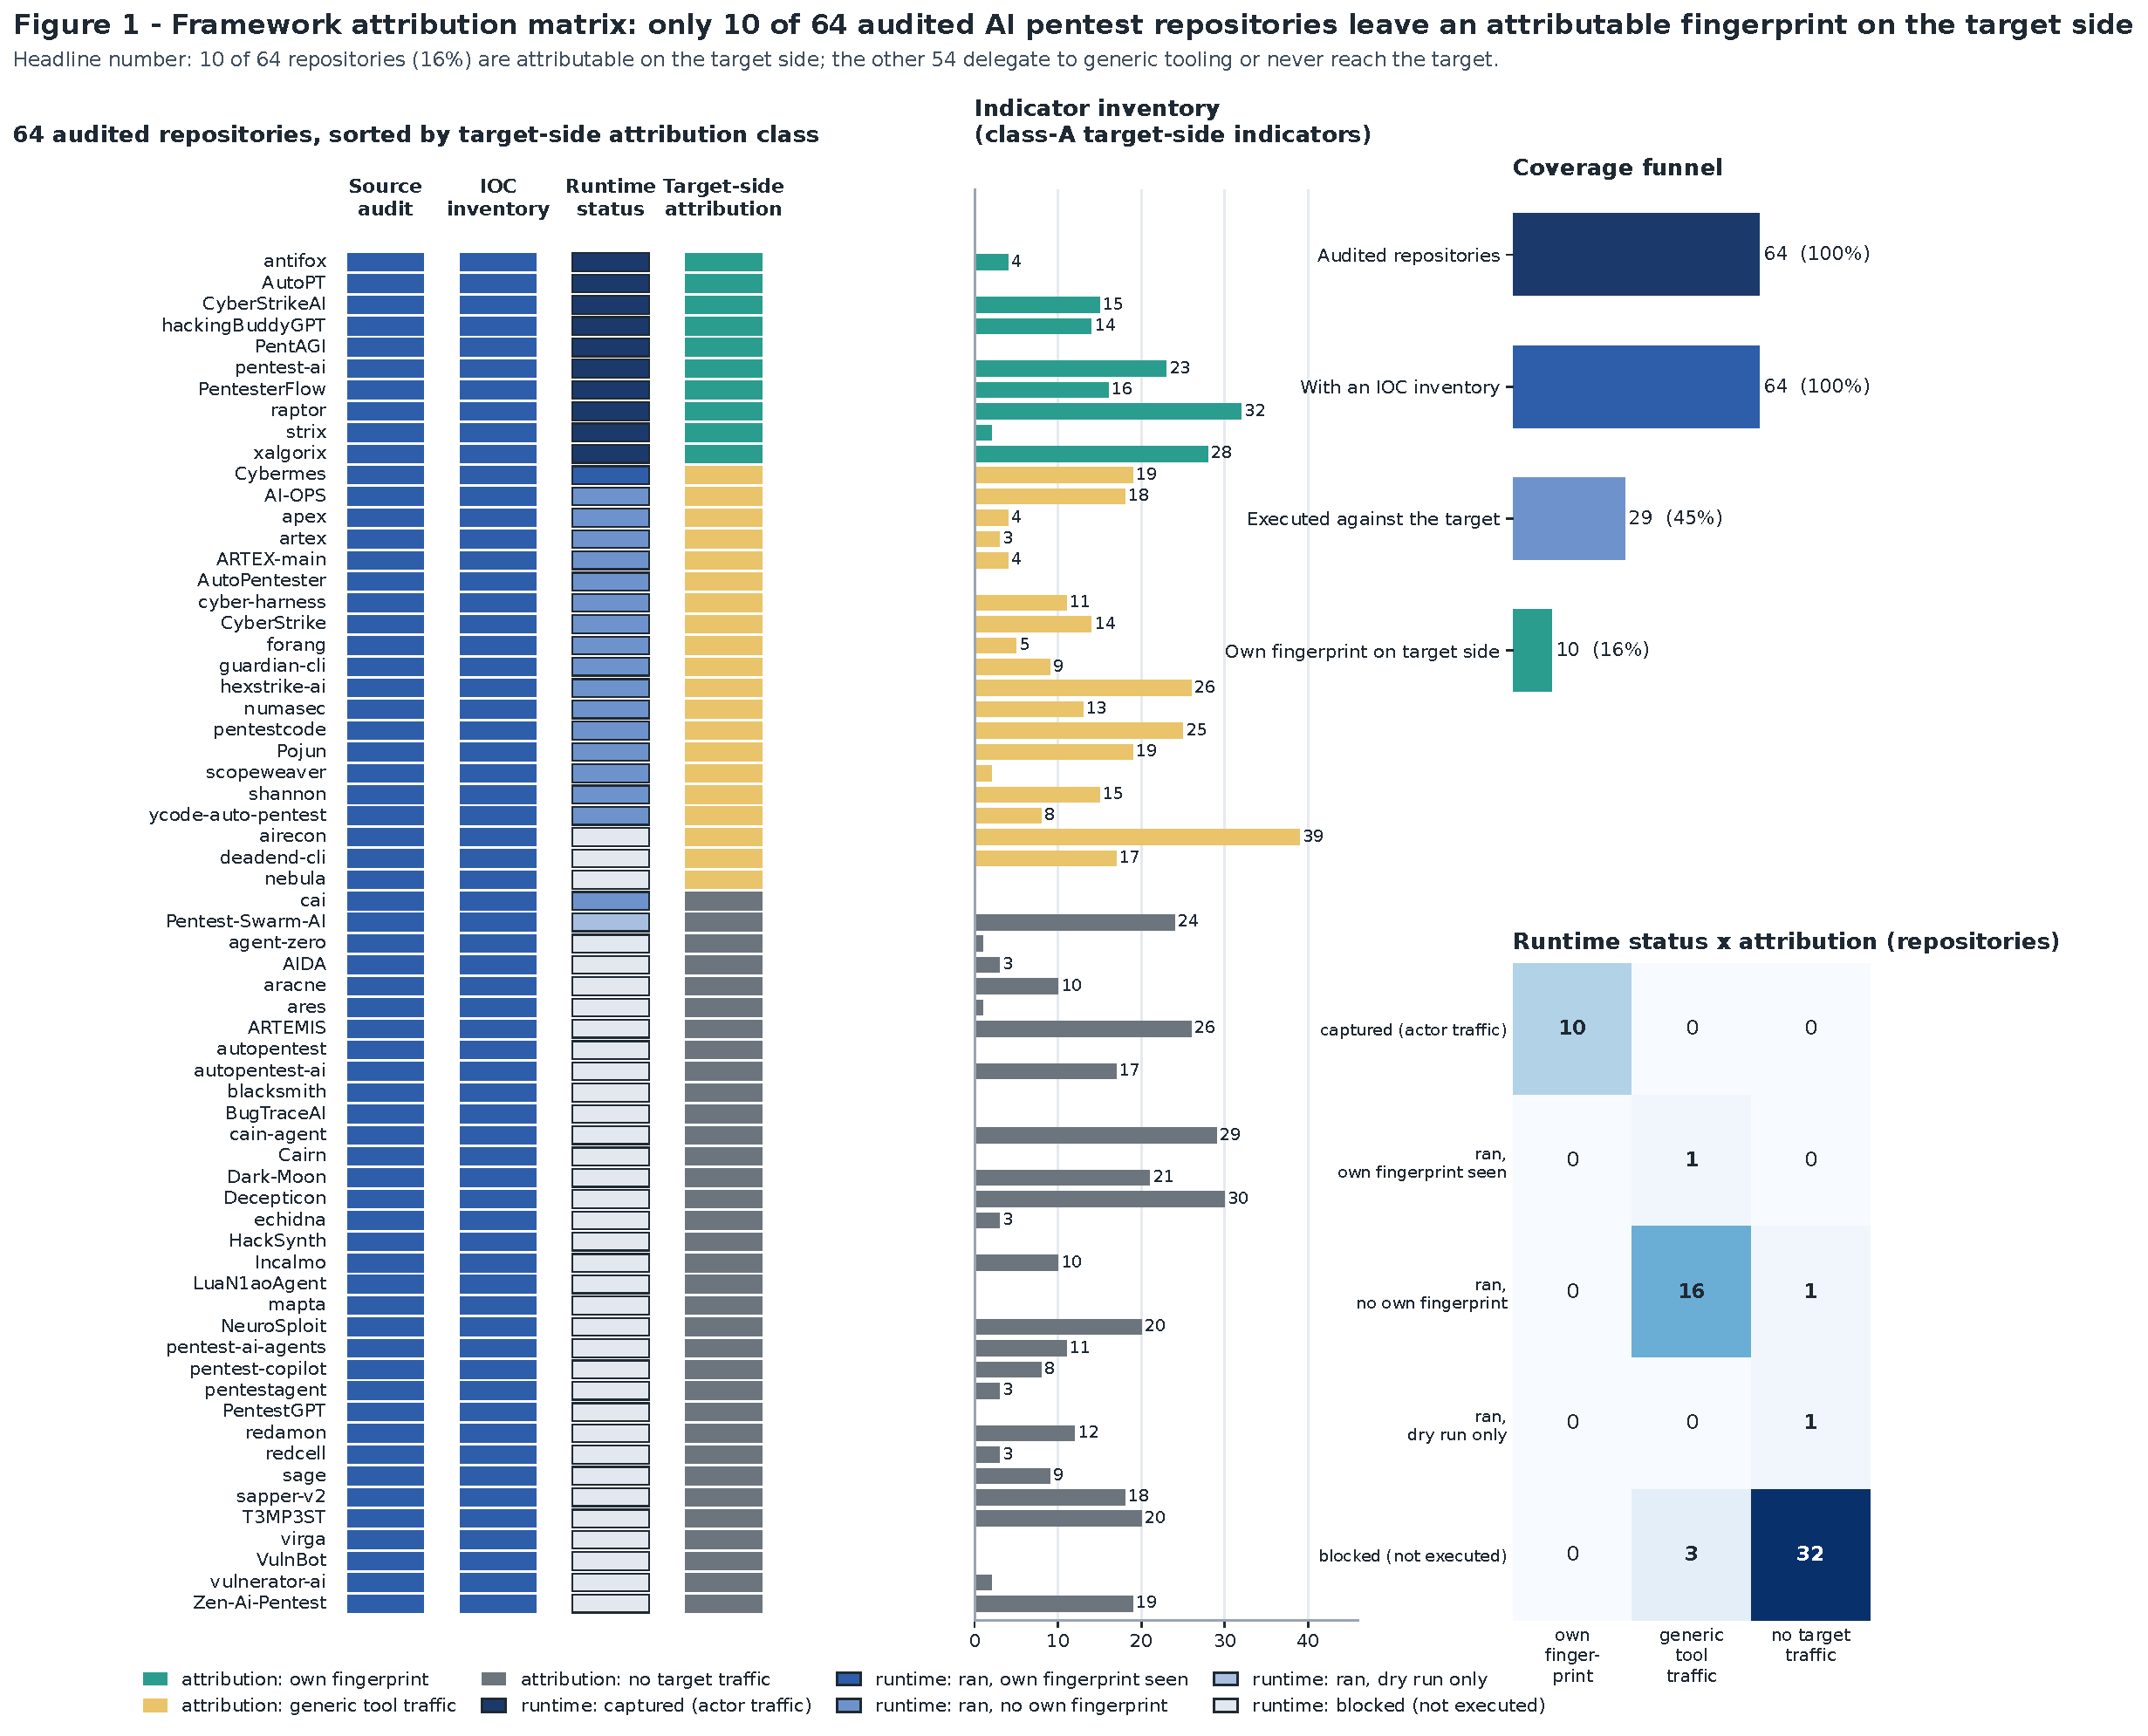
\includegraphics[trim=0 0 0 43bp,clip,width=0.76\textwidth]{figures/fig01_framework_attribution_matrix.pdf}
\caption{Framework attribution matrix: one row per audited AI pentest repository, with source
audit present, indicator inventory present, how far the runtime execution got, and whether the
framework leaves its own fingerprint on the target side (teal), only generic tool traffic
(amber) or no target traffic at all (grey).
\textbf{Headline: only 10 of the 64 audited repositories (16\%) are attributable on the target
side; 29 (45\%) could be executed against the evaluation target and 35 were blocked before
execution.}}
\label{fig:01}
\end{figure}

\textbf{Finding 2 --- source-code signatures need real-traffic qualification, and static
analysis cannot supply it.} Several strings that look like strong fingerprints are ordinary
client behaviour: a browser-disguise User-Agent, a bare \texttt{Python/3}, a
\texttt{True-Client-IP} header carrying a private address, a public out-of-band-interaction
domain. Each was verified by replaying the full rule set against 9.9 million real requests;
the surviving T1 set matches nothing in either real corpus.

\textbf{Finding 3 --- attribution is not detection.} Even perfect framework attribution does
not answer the operational question. We measure the false-positive rate of a behavioural
detector on 1,582 real attacker actors (2.72\%) and separately on six scanner actors
(66.67\%), and show that the latter is not a threshold-tuning problem: tool-driven traffic and
agent-driven traffic overlap in exactly the dimensions the detector measures.

The contributions are:
\begin{enumerate}
\item A source-audited corpus of 65 codebases (64 third-party frameworks plus one in-house
implementation) with a per-framework attribution matrix
(\ref{sec:framework}).
\item A tiered signature set of 610 rules with a documented derivation procedure, a
rule-usability screen, and zero hits on two real corpora (\ref{sec:tiers} and
\ref{sec:validation}).
\item An actor-level behavioural detector with an explicit fusion model and an algebraically
characterised decision rule (\ref{sec:actor}--\ref{sec:fusion}).
\item A quantified account of the attribution boundary, with three independent pieces of
evidence, and the deployment guidance that follows from it (\ref{sec:discussion} and
\ref{sec:limits}).
\item A released dataset and evaluation code, so every number in this paper can be recomputed
(\ref{sec:repro}).
\end{enumerate}

% =====================================================================
\section{Related Work}
\label{sec:related}

\textbf{Tool fingerprinting.} Signature-based attribution of security tooling is long
established in the honeypot and IDS literature. The problem this paper inherits is well known:
signatures derived from tool source code frequently match benign traffic, and the standard
remedy is empirical qualification against real captures. Our contribution here is to apply
that remedy at corpus scale and to report the resulting attrition explicitly, because the
attrition is the interesting result rather than an implementation detail.

\textbf{Attack detection.} Behavioural approaches to attack detection group requests into
sessions and score them against behavioural evidence. Our detector follows that line, with two
departures: the decision unit is the actor (source address plus time window) rather than the
session, and the evidence model is a noisy-OR with reverse evidence acting as a cap rather than
as a negative contribution.

\textbf{LLM agent detection.} Recent work distinguishes LLM-generated content from human
content in application-layer payloads. That setting is different in kind: the payload itself is
the signal. Here the interesting surface is \emph{request behaviour} --- the pattern of what an
agent probes next given what came back --- which is a much weaker signal than lexical markers.

\textbf{AI pentest frameworks.} Numerous open-source AI pentest agents have appeared since 2023.
They are typically evaluated on task success against vulnerable applications. That evaluation
is orthogonal to this work: we ask what the traffic looks like from the target side, including
when it looks like nothing distinctive at all.

% =====================================================================
\section{Threat Model and Problem Definition}
\label{sec:threat}

\subsection{Adversary setting}
\label{sec:adversary}

The adversary is an operator running an AI pentest agent against a protected asset. The
operator may be malicious. The agent may be one of the frameworks studied here, a commercial
product, or an in-house variant; the defensive measures must not assume any of them.

The defender operates a passive HTTP inspection point (reverse proxy, WAF, IDS) and may
additionally have egress logs from the same network segment.

\subsection{Objectives}
\label{sec:objectives}

\begin{table}[t]
\centering
\caption{The three objectives. A signature set addresses O1 only; O2 requires behaviour.}
\label{tab:objectives}
\begin{tabularx}{\textwidth}{@{}L{0.30\textwidth}Y@{}}
\toprule
\textbf{ID} & \textbf{Objective} \\
\midrule
\textbf{O1 (attribution)} & Given HTTP requests, determine which AI framework produced them \\
\textbf{O2 (detection)} & Given HTTP requests, determine whether an AI agent produced them \\
\textbf{O3 (operational)} & Keep the false-positive rate low enough to be deployable \\
\bottomrule
\end{tabularx}
\end{table}

O1 and O2 are distinct. A signature set addresses O1 only. O2 requires behaviour. Most of the
literature conflates them, which is one reason agent traffic is hard to operationalise.

\subsection{Non-goals}
\label{sec:nongoals}

We do not attempt to detect an agent's \emph{outbound} traffic to LLM providers; we describe it
in \ref{sec:egress} as the recommended complementary control but do not evaluate it. We do not
evaluate the frameworks' attack effectiveness. We do not claim the signature set is exhaustive
for any framework --- it reflects the audited revision, and \ref{sec:maintenance} discusses
maintenance.

% =====================================================================
\section{Evaluation Corpora}
\label{sec:corpora}

\begin{table}[t]
\centering
\caption{The six corpora used in this study. The two large corpora qualify the signature set;
the actor-level sets evaluate the behavioural detector.}
\label{tab:corpora}
\begin{tabularx}{\textwidth}{@{}L{0.26\textwidth}Y L{0.30\textwidth}@{}}
\toprule
\textbf{Corpus} & \textbf{Purpose} & \textbf{Size} \\
\midrule
\textbf{Framework corpus} (source) & Signature extraction & 65 repositories \\
\textbf{Live agent captures} (positive) & Detection evaluation & 15 actors / 12 frameworks / 211,547 requests \\
\textbf{Scanner captures} (negative) & Hard negative for tool-driven traffic & 6 actors / 999 requests \\
\textbf{Public internet traffic} & Rule false-positive validation & 9,905,794 requests / 80,987 source addresses \\
\textbf{WAF attack log} & Rule false-positive validation on attacks & 142,705 transactions / 30 days \\
\textbf{Real attacker actors} (negative) & Behavioural false-positive evaluation & 1,582 actors \\
\bottomrule
\end{tabularx}
\end{table}

The public internet traffic corpus is the public background-traffic dataset
\cite{burpheartbg}. The WAF attack log is a 30-day audit log produced by a ModSecurity
deployment running the OWASP Core Rule Set \cite{owaspcrs,modsecurity}. The two large corpora
are used only to qualify signatures. The behavioural detector is evaluated on the live captures
and on the two actor-level negative sets.

% =====================================================================
\section{Methodology}
\label{sec:method}

\subsection{The decision unit: the actor}
\label{sec:actor}

A single HTTP request carries very little evidence. \texttt{curl/8.23.0 GET /admin} is
produced by a human running curl, by a framework that shells out to curl, and by a
vulnerability scanner with the same defaults. Evidence accumulates only across a sequence of
requests, so the detector operates on the \textbf{actor}:

\begin{quote}
\itshape
An actor is the set of all requests from one source address within one time window.
\end{quote}

Two consequences follow. First, the alert unit becomes the source address rather than the
request, which is what an operator can actually act on. Second, the false-positive rate is
measured over actors, not requests --- a request-level false-positive rate would be misleading
by construction, since one noisy actor generates many requests. Every false-positive number in
this paper is actor-level.

The actor segmentation, the time-window length and the source-address grouping are implemented
once and shared by the collector, the feature extractor and the evaluator, so that no
measurement can drift between components.

\subsection{Feature families}
\label{sec:families}

Forty-three features are extracted from each actor's request sequence and grouped into ten
families (the shipped engine exposes 103 named features across 11 families). The families are
designed so that a family failure is diagnosable: each one isolates a different dimension of
agent behaviour.

\begin{table}[t]
\centering
\caption{The feature families used by the detector. The ablation over these families is
reported in \ref{sec:ablation}.}
\label{tab:families}
\begin{tabularx}{\textwidth}{@{}L{0.08\textwidth}L{0.22\textwidth}Y@{}}
\toprule
\textbf{Family} & \textbf{Dimension} & \textbf{Representative features} \\
\midrule
F3  & Post-error behaviour & error-to-endpoint-family switch rate, invalid-branch pruning rate, 404 tolerance \\
F4  & Breadth & distinct endpoint templates, distinct URL path segments \\
F5  & Exploration scale & endpoint templates per unit time, 4xx ratio, 2xx ratio, request rate \\
F6  & Enumeration and verification & ids enumerated per template, re-visit rate after a 2xx \\
F7  & Identity lineage & distinct identities used, unauthenticated ratio, identity churn \\
F8  & Session structure & requests per identity, parameter diversity \\
F9  & Execution channels & distinct User-Agent families in parallel use \\
F10 & Payload shape & request-body length distribution, content-type diversity \\
F13 & Dictionary-driven discrimination & configuration-path ratio (used as reverse evidence) \\
\bottomrule
\end{tabularx}
\end{table}

\subsection{Evidence rules}
\label{sec:evidence}

Fourteen evidence rules are implemented: twelve positive (E1--E12), two negative (E14, E15).
The identifier E13 is retired --- it was rejected on real traffic --- and E10 is a
response-side rule that cannot be computed from request data alone. Each rule carries a
weight $w$ that expresses how unlikely it is that a human produces the observed pattern --- it
is a diagnostic-likelihood ratio expressed as a prior-odds adjustment, not an accuracy claim.

\begin{table}[t]
\centering
\caption{Representative evidence rules. The complete table, with the exact conditions and
thresholds, is in the repository's \texttt{docs/METHODOLOGY.md} and in
\texttt{research/engine/evidence.py}.}
\label{tab:rules}
\begin{tabularx}{\textwidth}{@{}L{0.06\textwidth}R{0.09\textwidth}Y L{0.08\textwidth}@{}}
\toprule
\textbf{Rule} & \textbf{Weight} & \textbf{Condition} & \textbf{Family} \\
\midrule
E1  & 0.34 & explores many endpoint templates, continues despite a high 4xx ratio & F5 \\
E5  & 0.20 & after repeated errors, switches to a different endpoint family & F3 \\
E6  & 0.16 & abandons an invalid endpoint family entirely & F3 \\
E7  & 0.14 & enumerates ids within a single template & F6 \\
E9  & 0.12 & uses more than one execution channel (User-Agent family) in parallel & F9 \\
E11 & 0.12 & continues activity after 404 responses & F3 \\
E12 & 0.10 & revisits an endpoint after receiving a 2xx & F6 \\
E15 & 0.00 & dictionary-driven enumerator: high 4xx ratio, low 2xx rate, high template count & F13 \\
\bottomrule
\end{tabularx}
\end{table}

E10 carries a weight of 0.95 but is excluded from the fusion algebra because it depends on
response-side data that a passive collector does not have.

\subsection{Fusion and the decision rule}
\label{sec:fusion}

Positive evidence is fused with a noisy-OR model:
\[
  \mathrm{score}(\mathrm{actor}) \;=\; 1 - \prod_i \bigl(1 - w_i\bigr)
\]
over the positive rules that fire. The form is chosen for three properties: it is monotone in
every weight; it is the union bound of independent events, so weights are directly
interpretable as diagnostic strength; and it is trivially computable and auditable.

Figure~\ref{fig:02} shows the weight of each evidence rule and the conviction weight that a
whole feature family can reach on its own.

% source artwork: figures/fig09_evidence_rule_weights.pdf
\begin{figure}[t]
\centering
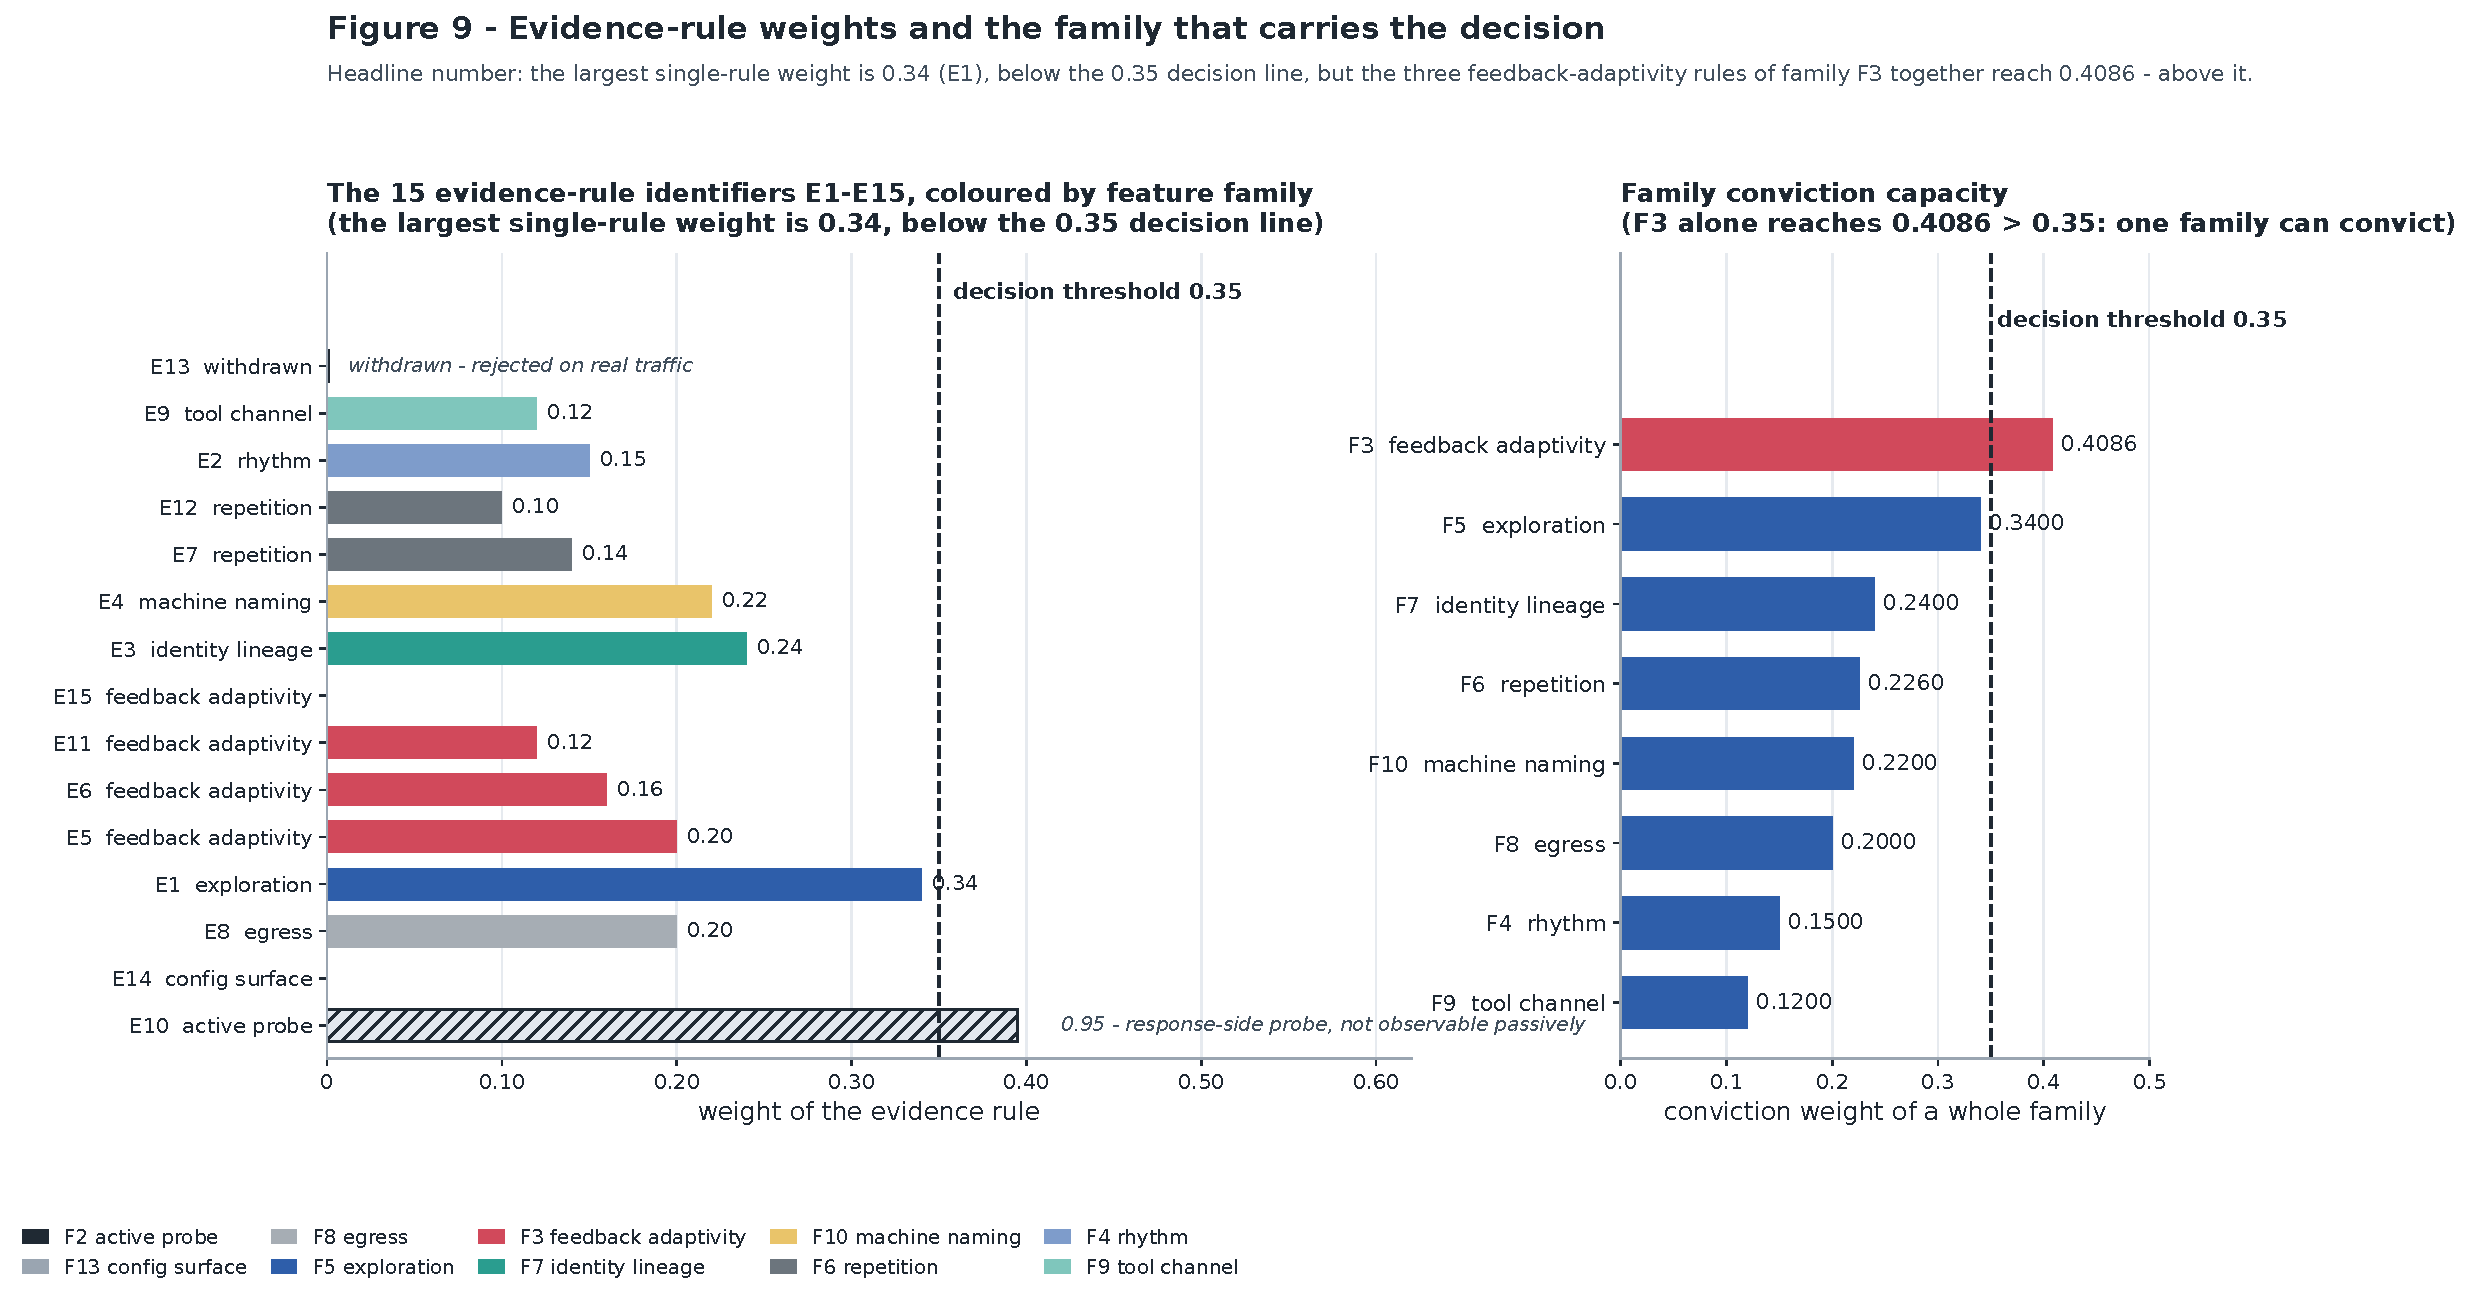
\includegraphics[trim=0 0 0 45.4bp,clip,width=0.88\textwidth]{figures/fig09_evidence_rule_weights.pdf}
\caption{Evidence-rule weights E1--E15 coloured by the feature family the rule reads, and the
conviction weight that a whole family can reach on its own. E10 (weight 0.95) needs
response-side data and is shown clipped; E13 was withdrawn after real-traffic validation.
\textbf{Headline: the largest single-rule weight is 0.34 (E1, exploration), below the 0.35
decision line, so no single rule can convict an actor; but the three feedback-adaptivity rules
of family F3 together reach 0.4086, i.e.\ above the decision line.}}
\label{fig:02}
\end{figure}

Negative rules do not enter the product. E15 instead acts as a \textbf{cap}: an actor matching
the dictionary-driven-automation profile is classified as non-agent regardless of how much
positive evidence it accumulates. This is deliberate. An agent running in a low-intensity mode,
or with a narrow scope, degenerates into dictionary enumeration, and at that point the actor's
traffic carries no information that distinguishes it from a human running the same dictionary
--- so scoring it as an agent would be wrong.

Three algebraic properties of the decision rule are worth stating, because they constrain what
the detector can and cannot do:

\begin{table}[t]
\centering
\caption{Algebraic properties of the decision rule.}
\label{tab:algebra}
\begin{tabularx}{\textwidth}{@{}L{0.30\textwidth}L{0.16\textwidth}Y@{}}
\toprule
\textbf{Property} & \textbf{Value} & \textbf{Consequence} \\
\midrule
Largest single-rule weight & 0.34 & Below the default threshold of 0.35, so \textbf{no single rule can convict} \\
Minimum convicting rule count & $k_{\min} = 2$ & At least two independent evidence rules must fire \\
Strongest single family & F3 at 0.40864 & \textbf{One family can convict} if all three of its rules fire \\
\bottomrule
\end{tabularx}
\end{table}

The middle row was initially reported incorrectly as 'a single family cannot convict'. The
correction matters: F3 alone reaches 0.40864, above the threshold, so the F3 family is
load-bearing in a way the others are not --- which the ablation in \ref{sec:ablation} confirms
empirically.

\subsection{Signature tiers and the rule-usability screen}
\label{sec:tiers}

Signature candidates are drawn from the audited source and verified line by line: a candidate
is admissible only if the recorded string is the literal value at the recorded file and line,
and only if the request scope is the target (as opposed to a third-party service, an LLM
provider, or the loopback interface).

Surviving candidates are then tiered. A rule is T1 only if it is framework-exclusive, has
target scope, is not a generic client behaviour, is not an attack semantic a human would also
produce, and \textbf{matches zero rules and zero actors across both real corpora}. T2 expresses
attack semantics without attribution value. T3 is generic tooling or over-broad and is excluded
from deployment.

Figure~\ref{fig:03} shows the composition of the tier-1 set by the request field that each
rule matches.

% source artwork: figures/fig02_t1_signature_composition.pdf
\begin{figure}[t]
\centering
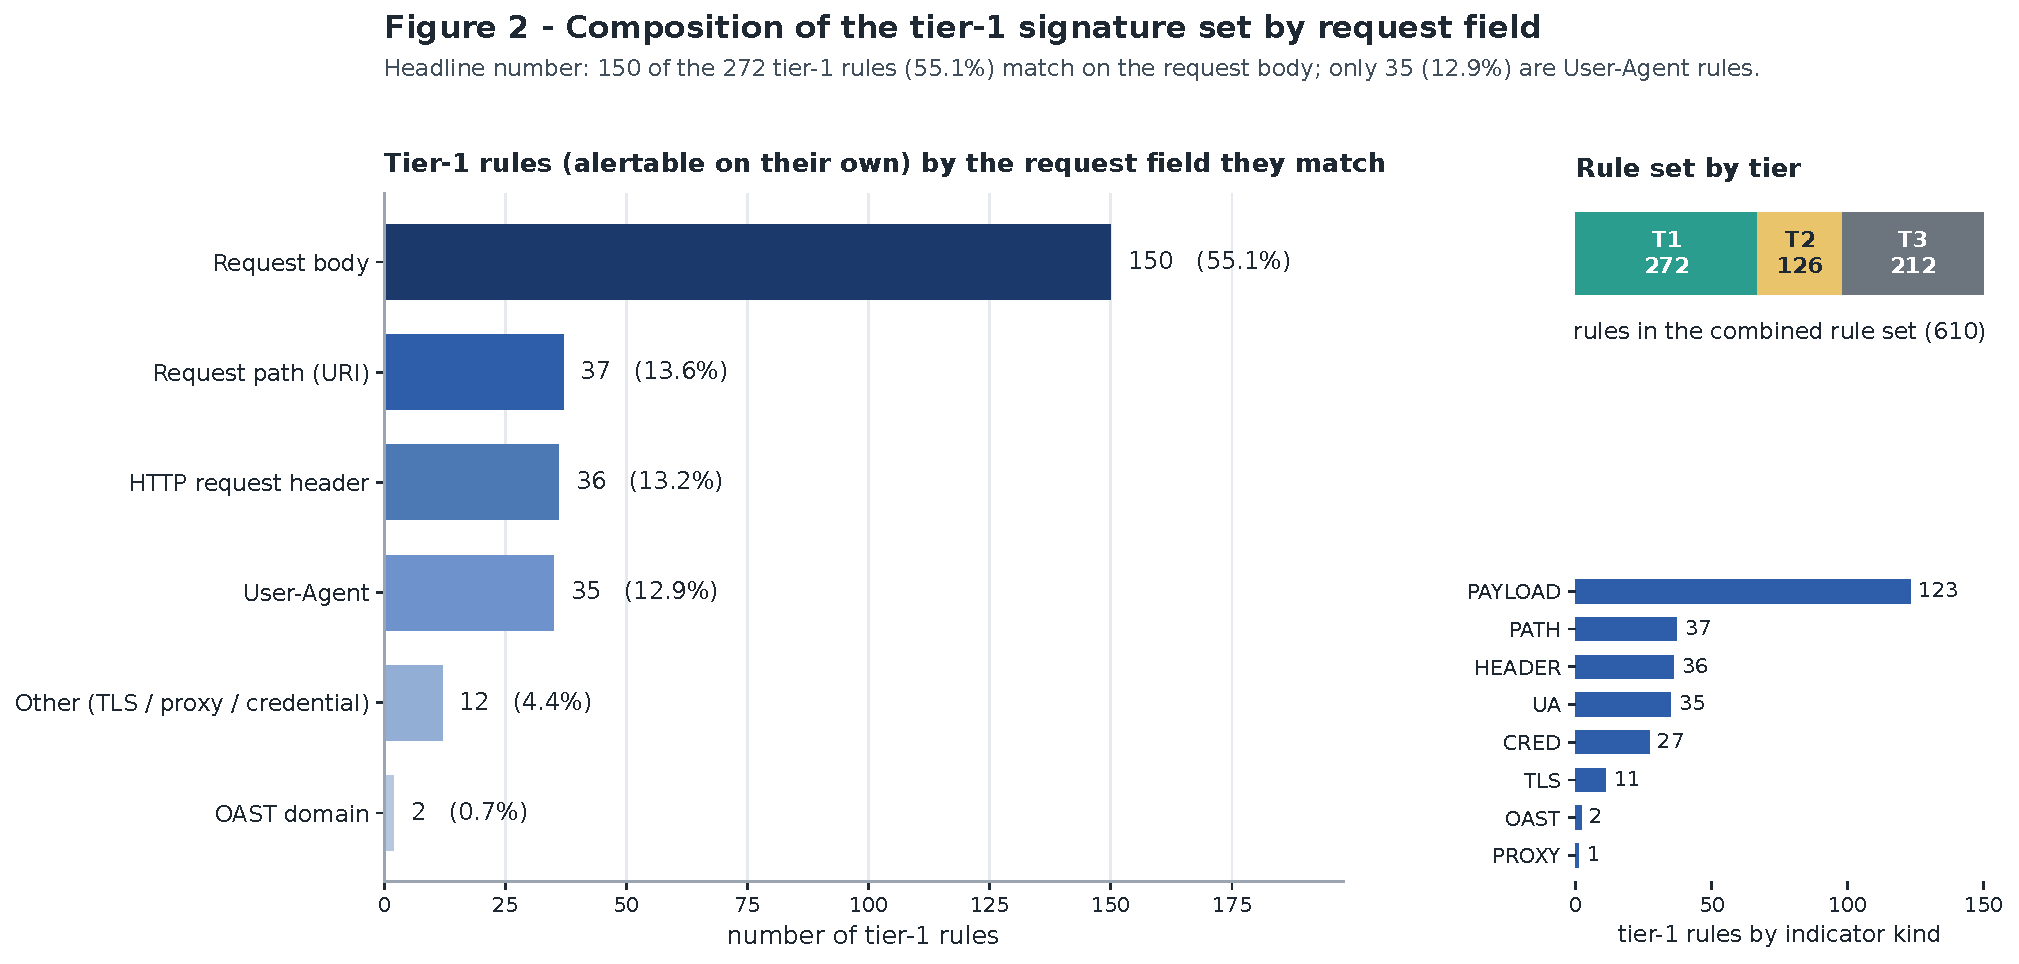
\includegraphics[trim=0 0 0 43.2bp,clip,width=0.88\textwidth]{figures/fig02_t1_signature_composition.pdf}
\caption{Composition of the tier-1 signature set by request field: the 272 tier-1 rules of the
combined 610-rule set (MIT 444 + AGPL 166) counted by the request field they match, next to the
tier split of the whole rule set.
\textbf{Headline: 150 of the 272 tier-1 rules (55.1\%) match on the request body, 37 (13.6\%)
on the request path, 36 (13.2\%) on a request header, 35 (12.9\%) on the User-Agent, 12 (4.4\%)
in other channels and 2 (0.7\%) on an OAST domain.}}
\label{fig:03}
\end{figure}

Static analysis cannot supply the last condition, and it is the condition that removes the most
rules. Six categories of candidate are discarded by a dedicated usability screen before
tiering:

\begin{table}[t]
\centering
\caption{The six categories of candidate removed by the rule-usability screen before tiering.}
\label{tab:screen}
\begin{tabularx}{\textwidth}{@{}L{0.22\textwidth}Y L{0.30\textwidth}@{}}
\toprule
\textbf{Category} & \textbf{Example} & \textbf{Disposition} \\
\midrule
Source-code templates & \texttt{f"/\{path[0]\}/1/\{path[2]\}"} & T3 --- the emitted request carries the evaluated value, not the template \\
Descriptive text mixed into the literal & a literal prefixed with a non-ASCII descriptive phrase & T3 --- cannot match real traffic \\
Placeholder tokens & \texttt{https://\{target\}/graphql} & T3 \\
Example hostnames & \texttt{X-Forwarded-Host: attacker.com} & T3 \\
Generic credentials and command templates & \texttt{admin:admin}, \texttt{nc -e /bin/bash attacker.com} & T2 --- a human sends the same thing \\
Identifier lists and prototype-pollution payloads & \texttt{com.opensymphony.\allowbreak xwork2.\allowbreak ActionContext / ...} & T2 \\
\bottomrule
\end{tabularx}
\end{table}

The screen removed 68 rules that were otherwise plausible. Several of them would have been
deployed as strong signals and would have produced no detections at all.

\subsection{Signature matching semantics}
\label{sec:matching}

Generation, validation and export share one implementation of the matching semantics. A
literal is escaped, \texttt{*} becomes a wildcard that cannot cross whitespace or a path
separator, and the resulting expression is normalised for the target platform (notably,
\texttt{\textbackslash s} is not supported by the Lucene-style query languages and is
replaced). Sharing one implementation is not a stylistic choice: earlier versions of this work
shipped deployable files whose validation semantics differed from the generator's, and the
failure was only caught because the exported files were counted rather than parsed.

% =====================================================================
\section{Framework Corpus and Audit Procedure}
\label{sec:framework}

\subsection{Corpus}
\label{sec:corpus}

The corpus comprises 65 audited codebases --- 64 third-party frameworks plus one in-house
implementation --- selected to span the designs that actually exist rather than a single
architectural family: prompt-driven agents, orchestrated tool-calling agents, multi-agent
pipelines, and skill-library designs. The audit recorded, for each framework, the
request-sending code paths and the strings they emit.

\subsection{Audit procedure}
\label{sec:audit}

Each framework is audited statically. For every candidate string the auditor records the file
and line, the request scope (target, third-party service, LLM provider, loopback), whether the
call site is live or dead, and the attack stage at which it is emitted. Three classes of
string are systematically excluded and reported separately: values appearing only in test
fixtures, documentation and demo data; values with no live call site; and generic tooling
identifiers (curl, wget, python-requests, Go-http-client, ffuf, nuclei, httpx, sqlmap, browser
User-Agents). The last group is reported rather than discarded, because knowing which
frameworks are \emph{only} observable through generic tooling is itself a finding.

\subsection{Attribution matrix}
\label{sec:matrix}

The matrix in the repository's \texttt{docs/FRAMEWORK\_COVERAGE.md} records, per framework,
whether it emits its own identifying request, whether it is attributable on the target side,
how it was validated, and --- where it could not be run --- the specific blocker.

Figure~\ref{fig:01}, shown in the introduction, gives the full attribution matrix.
The headline numbers:

\begin{table}[t]
\centering
\caption{Headline attribution numbers. The gap between 41 and 10 is the single most important
number in this paper.}
\label{tab:attribution}
\begin{tabularx}{\textwidth}{@{}Y R{0.18\textwidth}@{}}
\toprule
\textbf{Category} & \textbf{Count} \\
\midrule
Codebases audited (64 third-party frameworks + 1 in-house) & 65 \\
Frameworks with T1 source-level signatures & 41 framework labels \\
\textbf{Frameworks validated end-to-end as attributable on the target side} & \textbf{10} \\
Frameworks whose target-side traffic is entirely generic tool traffic & 18 (run and inspected) \\
Frameworks that cannot produce HTTP target traffic at all, or could not be executed & remainder \\
\bottomrule
\end{tabularx}
\end{table}

The gap between 41 and 10 is the single most important number in this paper. Forty-one
frameworks contain a string that could, in principle, identify them --- but for most of them
that string never reaches the victim, because the framework's HTTP client is used to talk to
its own tooling or to an LLM provider, not to the target.

% =====================================================================
\section{Results}
\label{sec:results}

\subsection{Signature validation on real traffic}
\label{sec:validation}

\begin{table}[t]
\centering
\caption{Tier-1 signature validation on the two real corpora.}
\label{tab:validation}
\begin{tabularx}{\textwidth}{@{}Y L{0.40\textwidth} R{0.16\textwidth}@{}}
\toprule
\textbf{Corpus} & \textbf{Requests / transactions} & \textbf{T1 rules matched} \\
\midrule
Public internet traffic & 9,905,794 requests, 80,987 source addresses & \textbf{0} \\
Real WAF attack transactions (30 days) & 142,705 & \textbf{0} \\
\bottomrule
\end{tabularx}
\end{table}

% source artwork: figures/fig08_rule_validation_real_traffic.pdf
\begin{figure}[t]
\centering
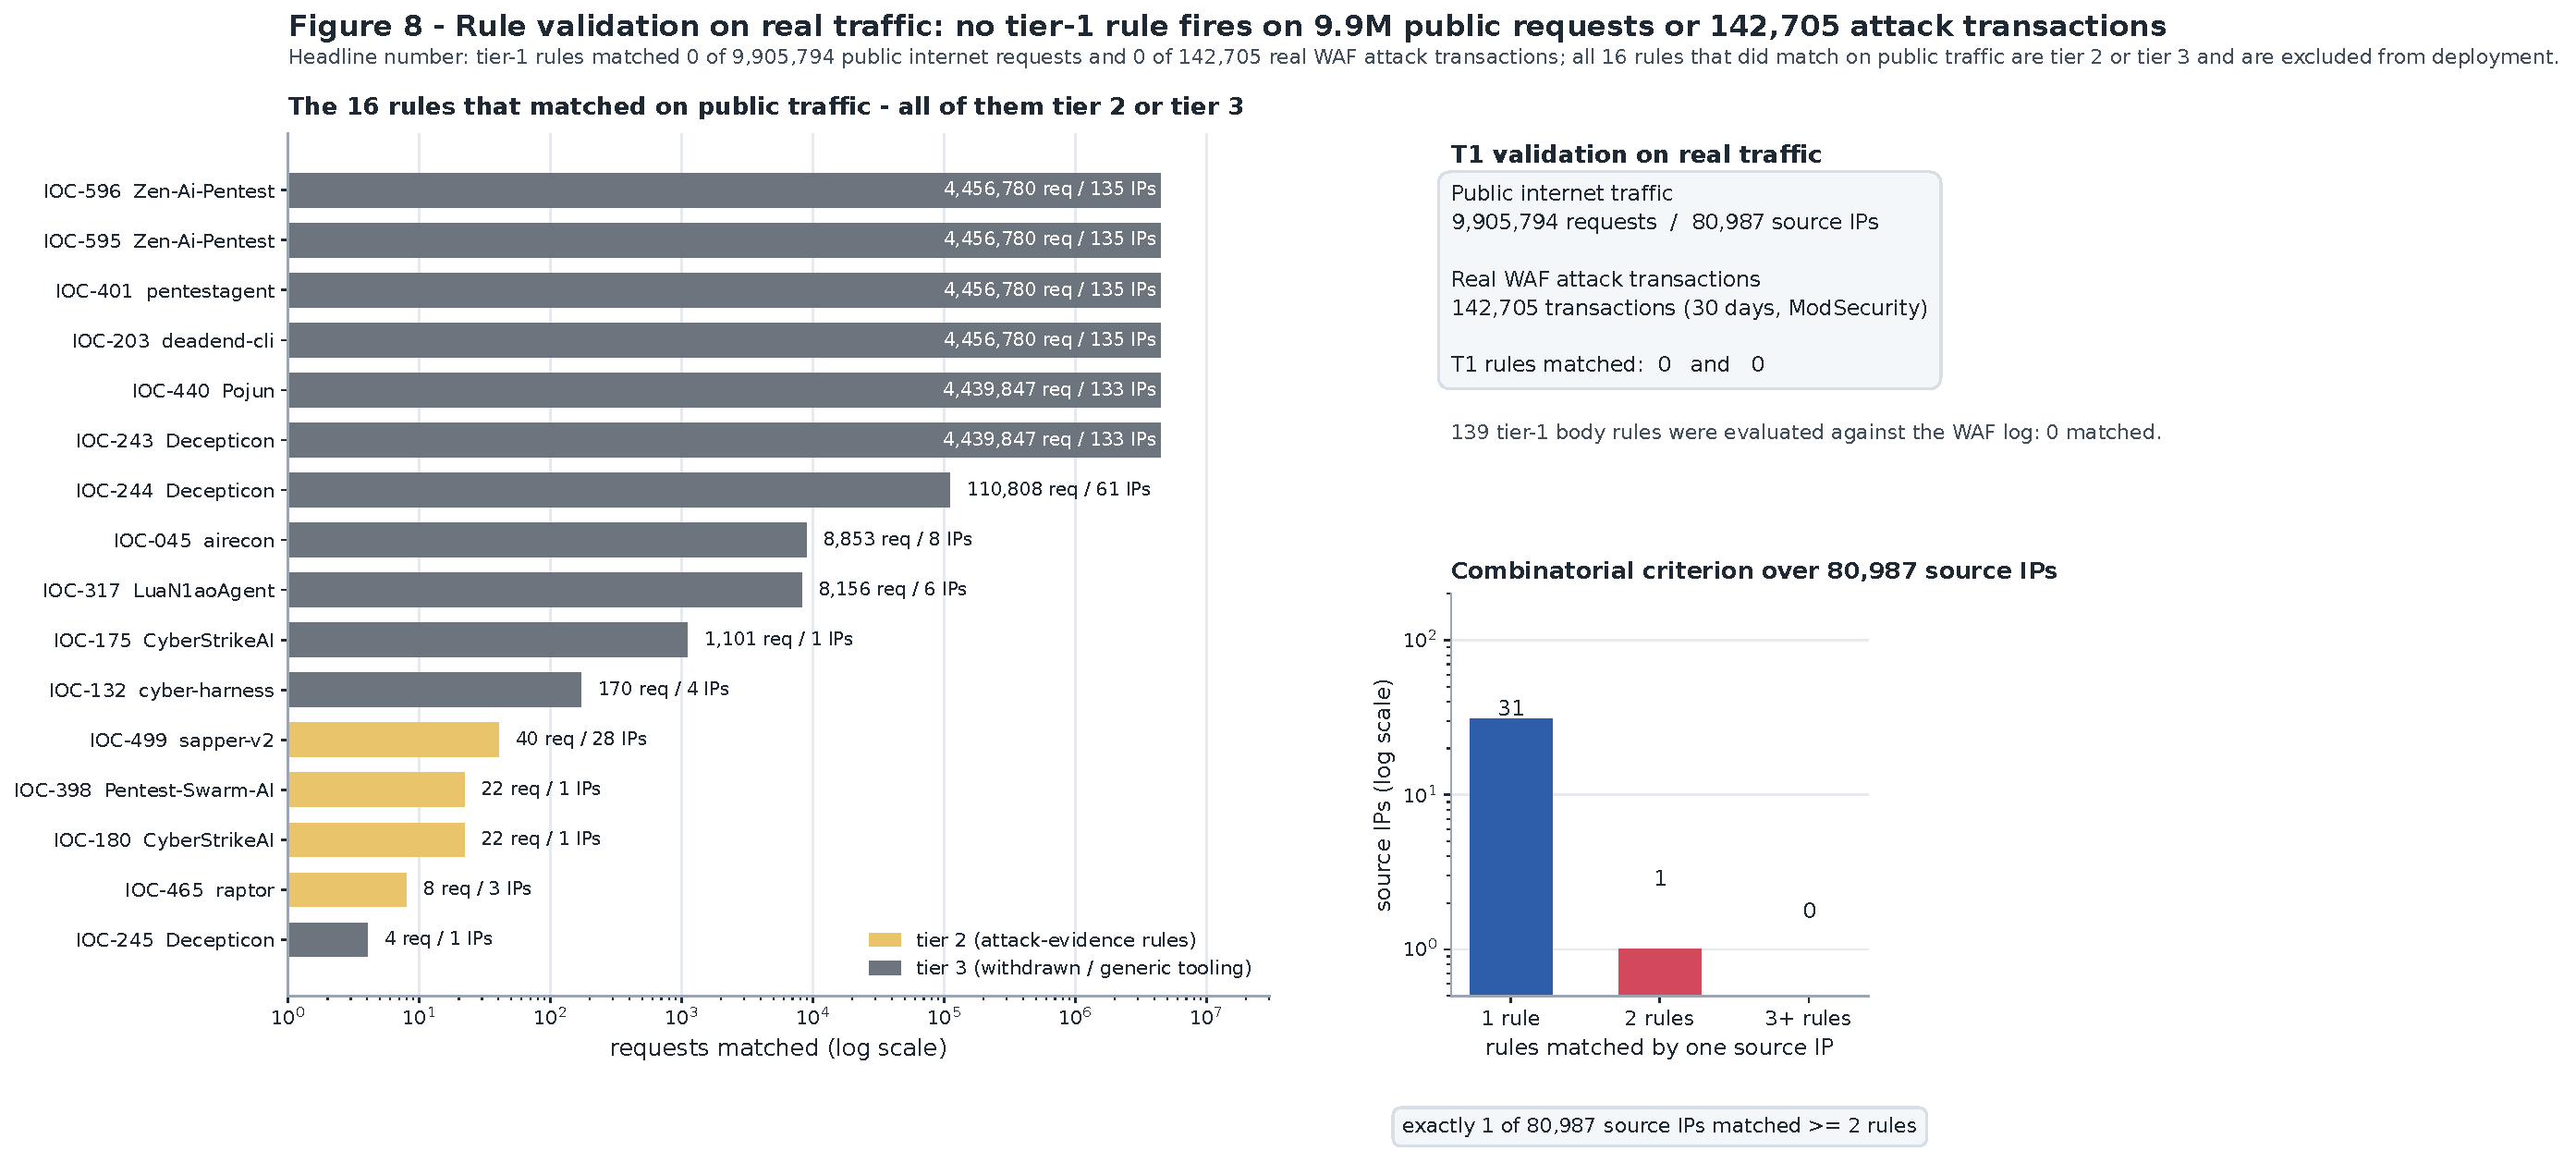
\includegraphics[trim=0 0 0 39.7bp,clip,width=0.88\textwidth]{figures/fig08_rule_validation_real_traffic.pdf}
\caption{Rule validation on real traffic: the 16 rules that matched on 9,905,794 public internet
requests, the tier-1 validation result for the public-traffic scan and for the 30-day
ModSecurity WAF audit log, and the number of source addresses that matched one, two or more
rules.
\textbf{Headline: tier-1 rules matched 0 of 9,905,794 public requests (80,987 source IPs) and
0 of 142,705 real WAF attack transactions; all 16 rules that did match on public traffic are
tier 2 or tier 3, and exactly 1 of the 80,987 source addresses matched 2 or more rules (31
matched exactly one).}}
\label{fig:04}
\end{figure}

Figure~\ref{fig:04} gives the validation result in full: which rules matched, at which
tier, and how many source addresses matched one, two or more rules.

Sixteen rules matched on the public corpus \cite{burpheartbg}. Every one is T2 or T3:
browser-disguise User-Agents, a bare \texttt{Python/3}, a public out-of-band-interaction
domain, generic payload markers. None is deployable for attribution, and none is included in
the released T1 set.

Under the combinatorial criterion --- one source address matching at least two T1 rules --- the
public corpus yields exactly \textbf{one} flagged address out of 80,987.

\subsection{Behavioural detection}
\label{sec:detection}

\begin{table}[t]
\centering
\caption{Behavioural detection results on the 15 live AI-agent captures covering 12
frameworks.}
\label{tab:detection}
\begin{tabularx}{\textwidth}{@{}Y L{0.34\textwidth}@{}}
\toprule
\textbf{Metric} & \textbf{Value} \\
\midrule
Actors & 15 live AI-agent captures, 12 frameworks \\
Segment recall at threshold 0.35 & \textbf{13/15 = 86.7\%} \\
Framework recall & \textbf{10/12 = 83.3\%} \\
Framework-level one-sided 95\% lower bound & \textbf{0.779} ($0.05^{1/12}$) \\
Per-actor scores & 0.803 (DSH) down to 0.250 (pentest-ai) \\
\bottomrule
\end{tabularx}
\end{table}

Figure~\ref{fig:05} gives the per-segment attribution score against the decision
threshold, and Figure~\ref{fig:06} shows the duration and the request volume of each of the
15 captures.

% source artwork: figures/fig03_per_framework_detection_score.pdf
\begin{figure}[t]
\centering
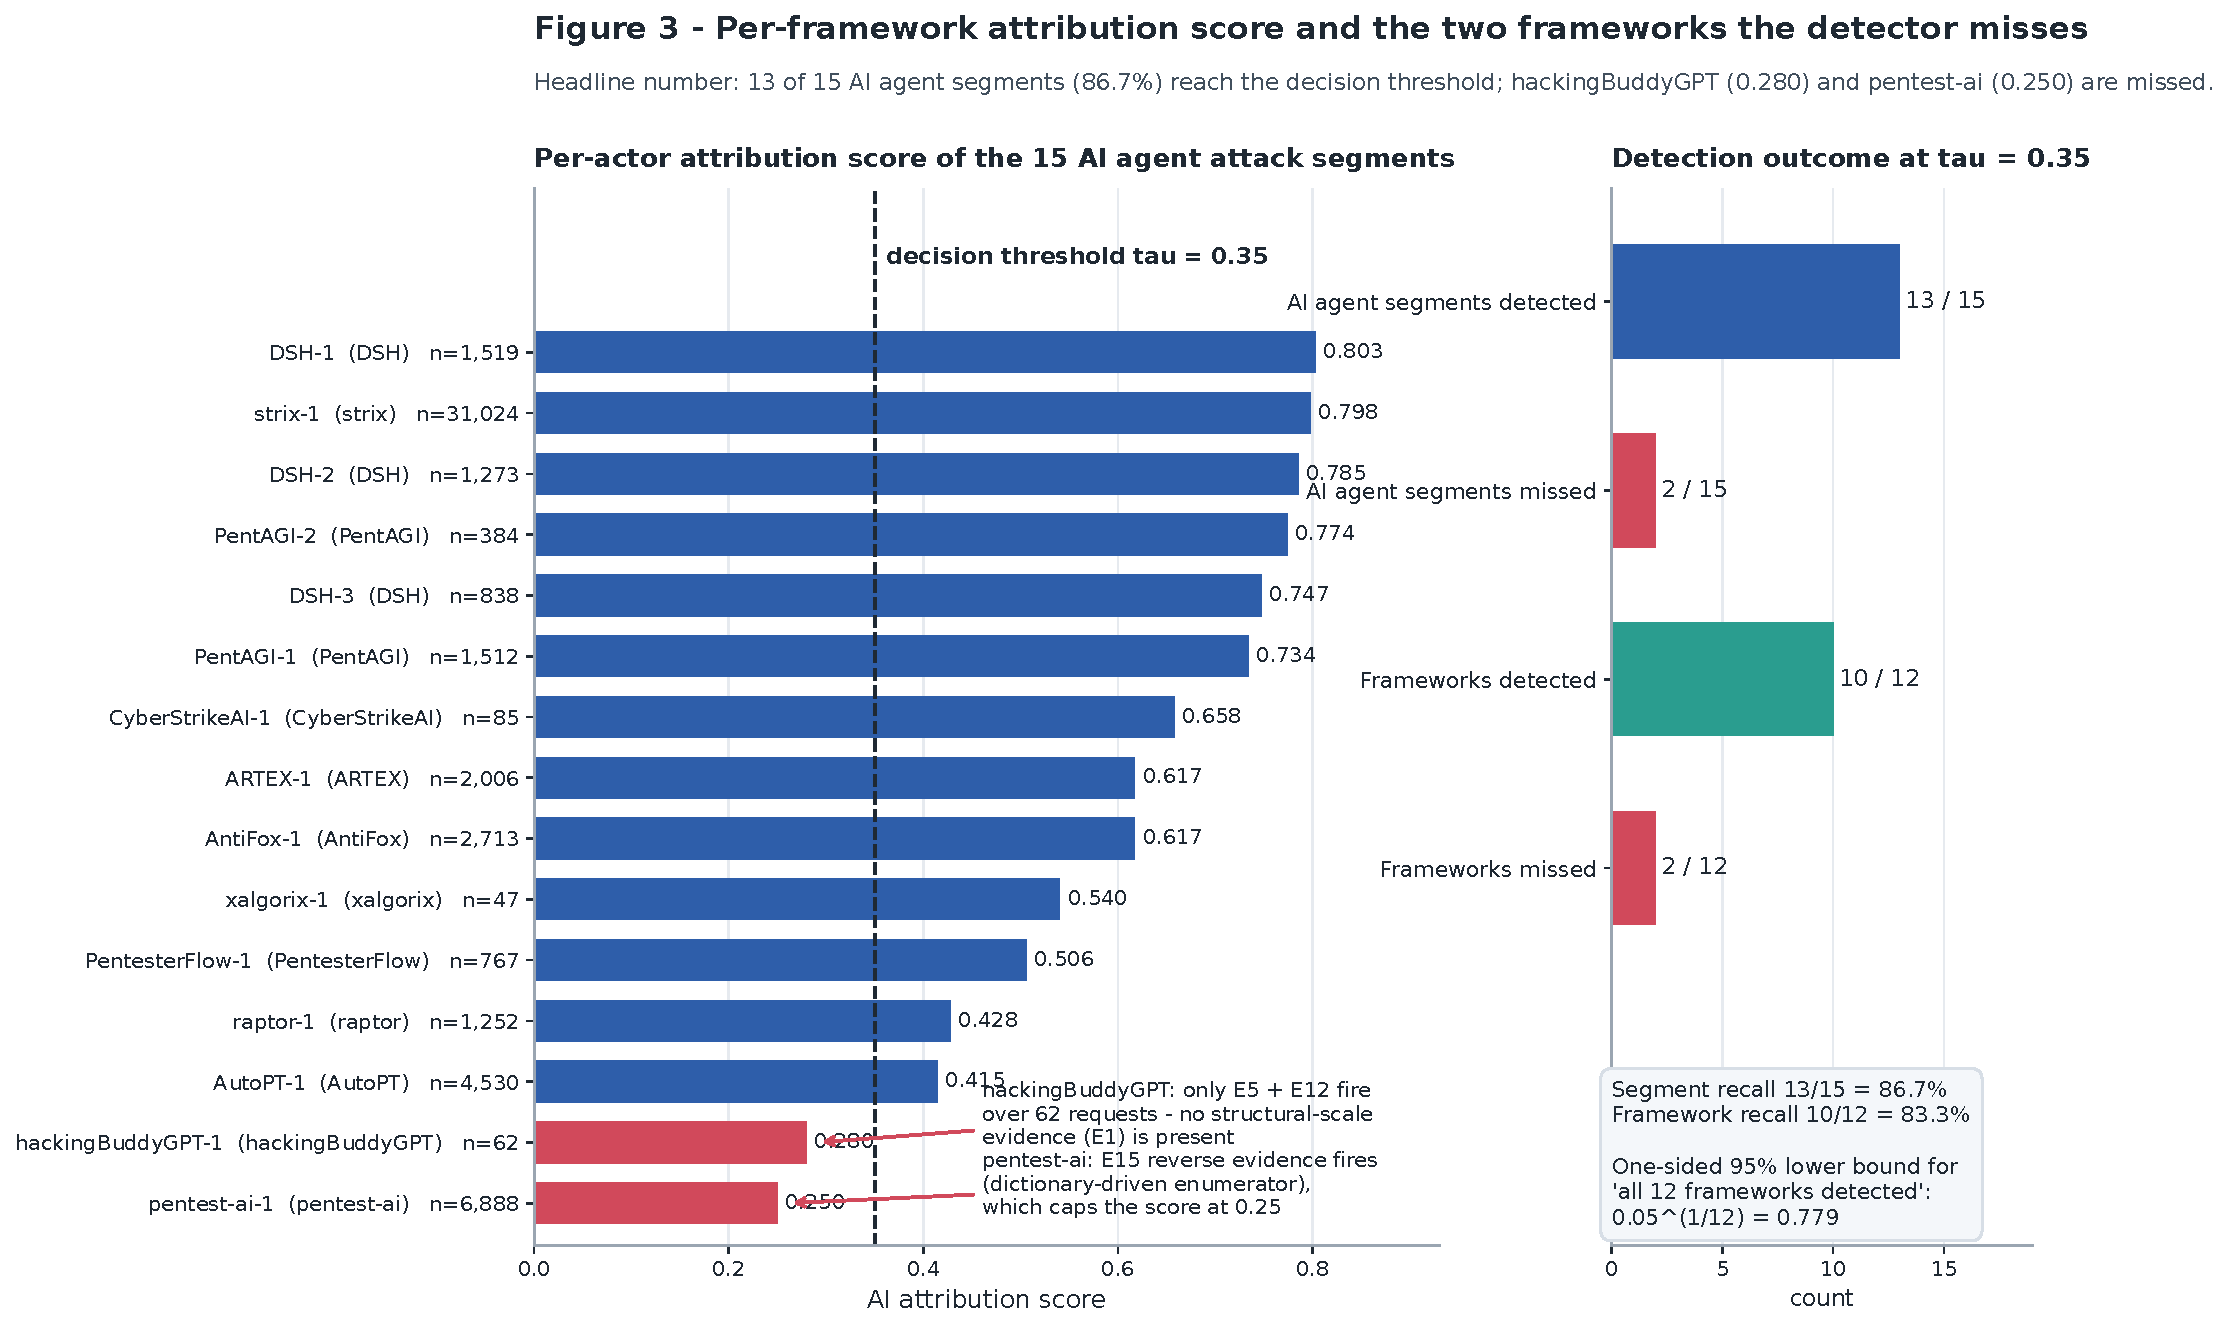
\includegraphics[trim=0 0 0 49.7bp,clip,width=0.88\textwidth]{figures/fig03_per_framework_detection_score.pdf}
\caption{Per-framework attribution score of the 15 AI agent attack segments against the decision
threshold $\tau = 0.35$, with the request count of each segment.
\textbf{Headline: 13 of 15 segments (86.7\%) and 10 of 12 frameworks (83.3\%) reach
$\tau = 0.35$; the two misses are hackingBuddyGPT (0.280, only E5 and E12 fire) and pentest-ai
(0.250, vetoed by the E15 reverse-evidence rule); the one-sided 95\% lower bound for 'all 12
frameworks detected' is $0.05^{1/12} = 0.779$.}}
\label{fig:05}
\end{figure}

% source artwork: figures/fig11_ai_actor_timeline.pdf
\begin{figure}[t]
\centering
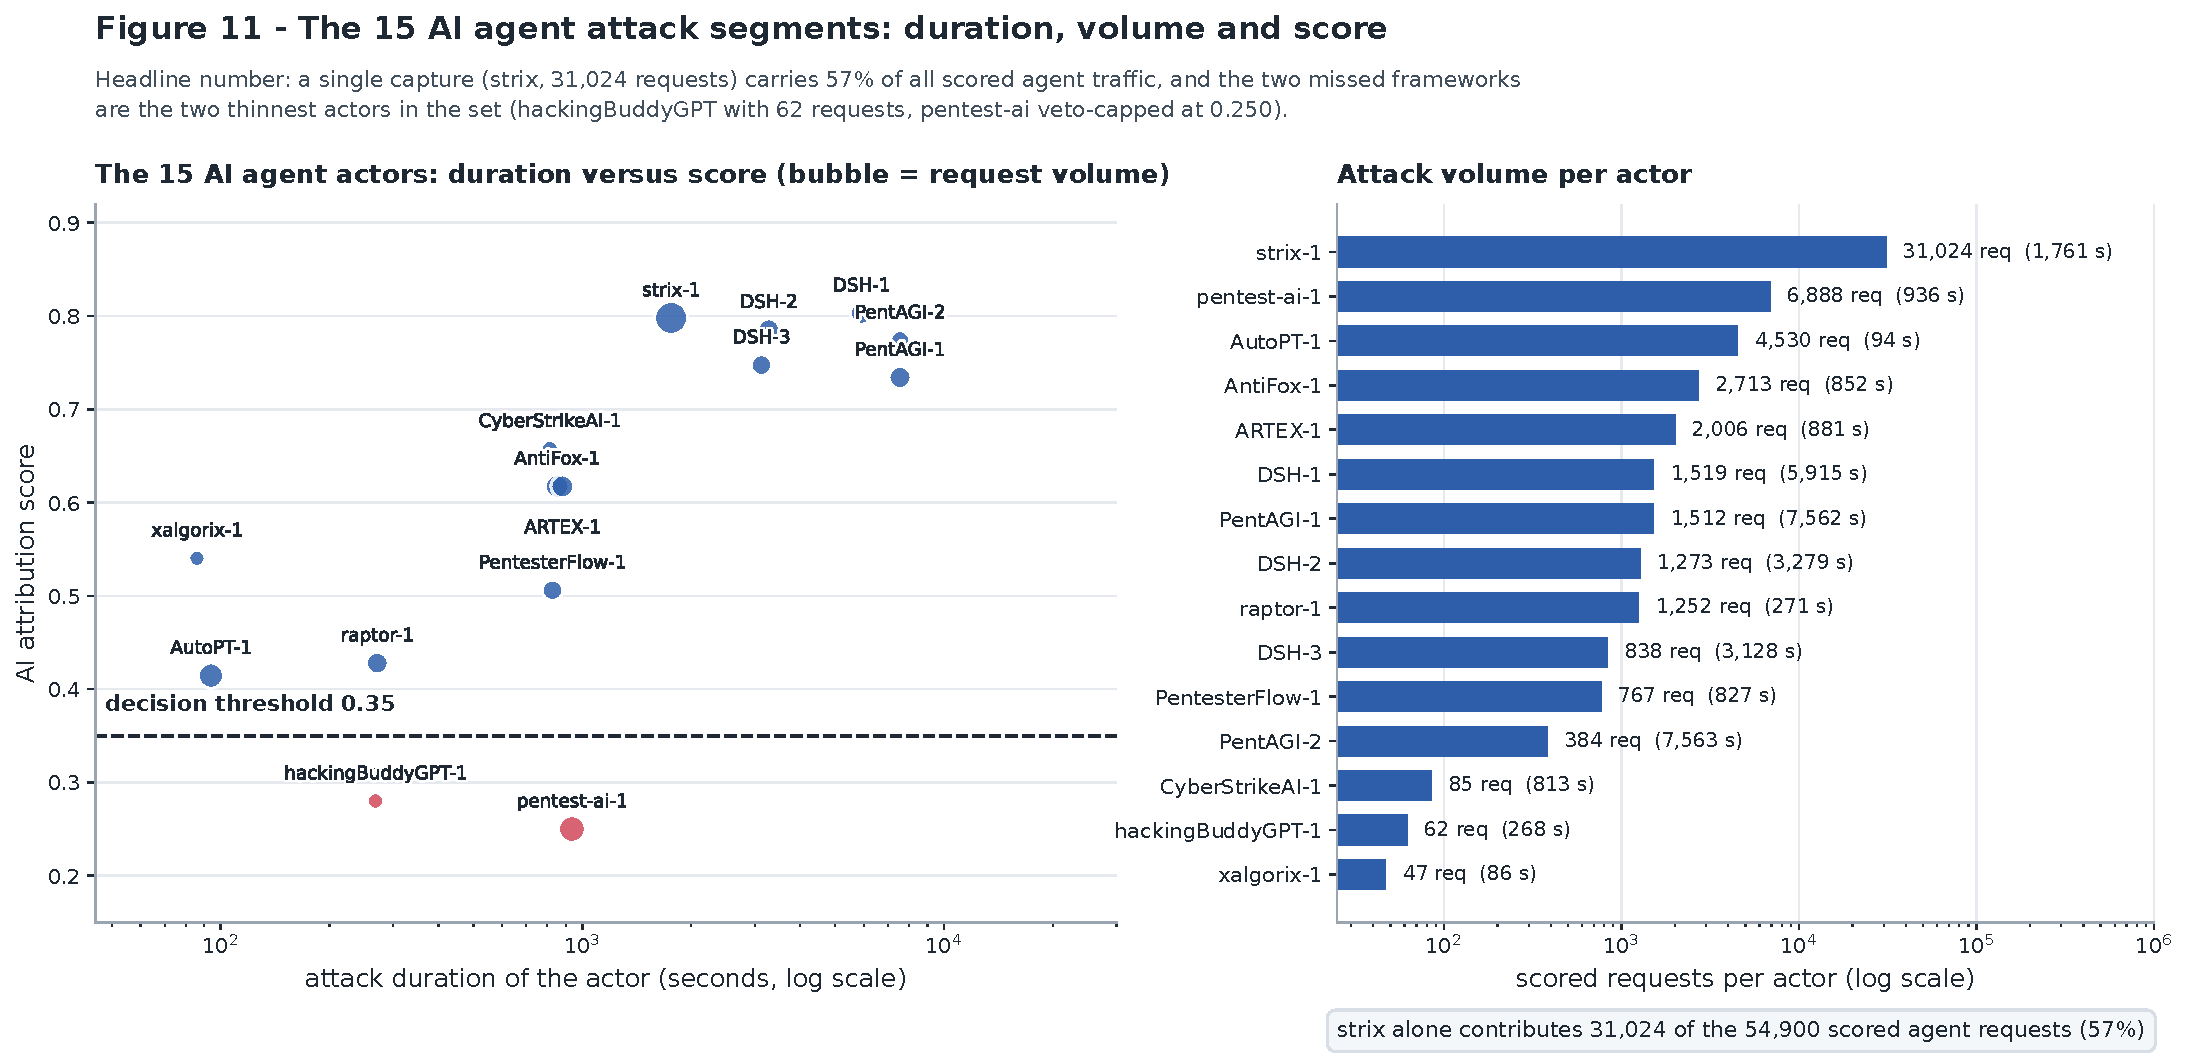
\includegraphics[trim=0 0 0 62.8bp,clip,width=0.88\textwidth]{figures/fig11_ai_actor_timeline.pdf}
\caption{The 15 AI agent attack segments: attack duration against attribution score with the
bubble area showing the request volume, and the scored request volume per actor.
\textbf{Headline: a single capture (strix, 31,024 of the 54,900 scored agent requests, 57\%)
carries more than half of all scored agent traffic, and the two missed frameworks are the two
thinnest actors in the set (hackingBuddyGPT with 62 requests, pentest-ai veto-capped at
0.250).}}
\label{fig:06}
\end{figure}

Clopper-Pearson and Jeffreys intervals over the segment-level proportion are reported in the
repository's \texttt{docs/RESULTS.md}.

\subsection{False positives}
\label{sec:falsepositives}

\begin{table}[t]
\centering
\caption{False-positive rates on the two actor-level negative sets, at threshold 0.35.}
\label{tab:fp}
\begin{tabularx}{\textwidth}{@{}Y R{0.13\textwidth} R{0.17\textwidth} L{0.26\textwidth}@{}}
\toprule
\textbf{Negative set} & \textbf{Actors} & \textbf{False positives} & \textbf{FPR} \\
\midrule
Real attackers (WAF-derived) & 1,582 & 43 & \textbf{2.72\%} (95\% CI [2.02\%, 3.64\%]) \\
Scanner actors & 6 & 4 & \textbf{66.67\%} \\
\bottomrule
\end{tabularx}
\end{table}

Figure~\ref{fig:07} shows the recall and false-positive trade-off across the decision
threshold, with the chosen operating point marked on both panels; Figure~\ref{fig:08} breaks
the false-positive rate down by negative population.

% source artwork: figures/fig04_threshold_tradeoff.pdf
\begin{figure}[t]
\centering
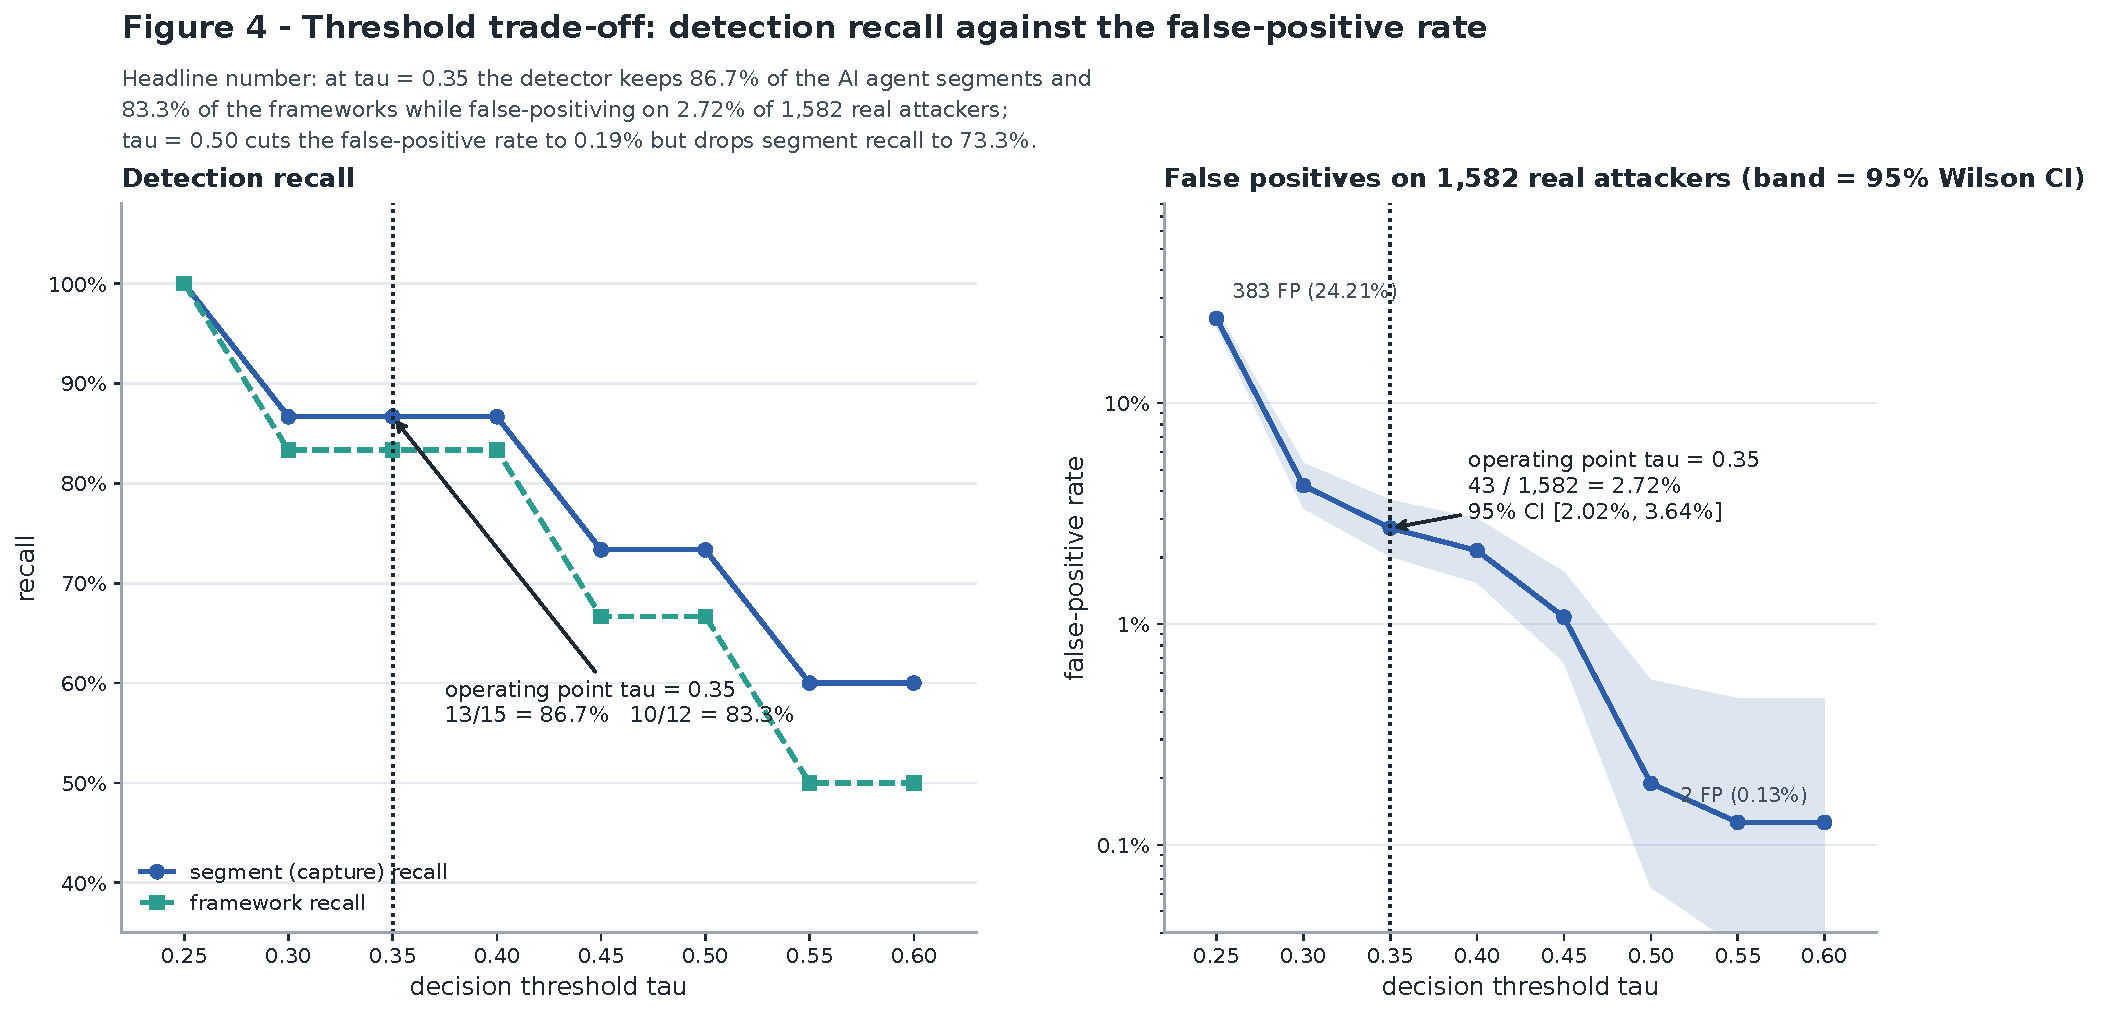
\includegraphics[trim=0 0 0 75.9bp,clip,width=0.88\textwidth]{figures/fig04_threshold_tradeoff.pdf}
\caption{Threshold trade-off: segment and framework recall as a function of the decision
threshold, and the false-positive rate on the 1,582 real attacker actors with its 95\% Wilson
interval, on a log scale. The chosen operating point is marked on both panels.
\textbf{Headline: at $\tau = 0.35$ the detector keeps 86.7\% of the segments and 83.3\% of the
frameworks while false-positiving on 43 of 1,582 real attackers (2.72\%, 95\% CI
2.02--3.64\%); $\tau = 0.50$ lowers the false-positive rate to 0.19\% but drops segment recall to
73.3\%.}}
\label{fig:07}
\end{figure}

% source artwork: figures/fig05_false_positive_breakdown.pdf
\begin{figure}[t]
\centering
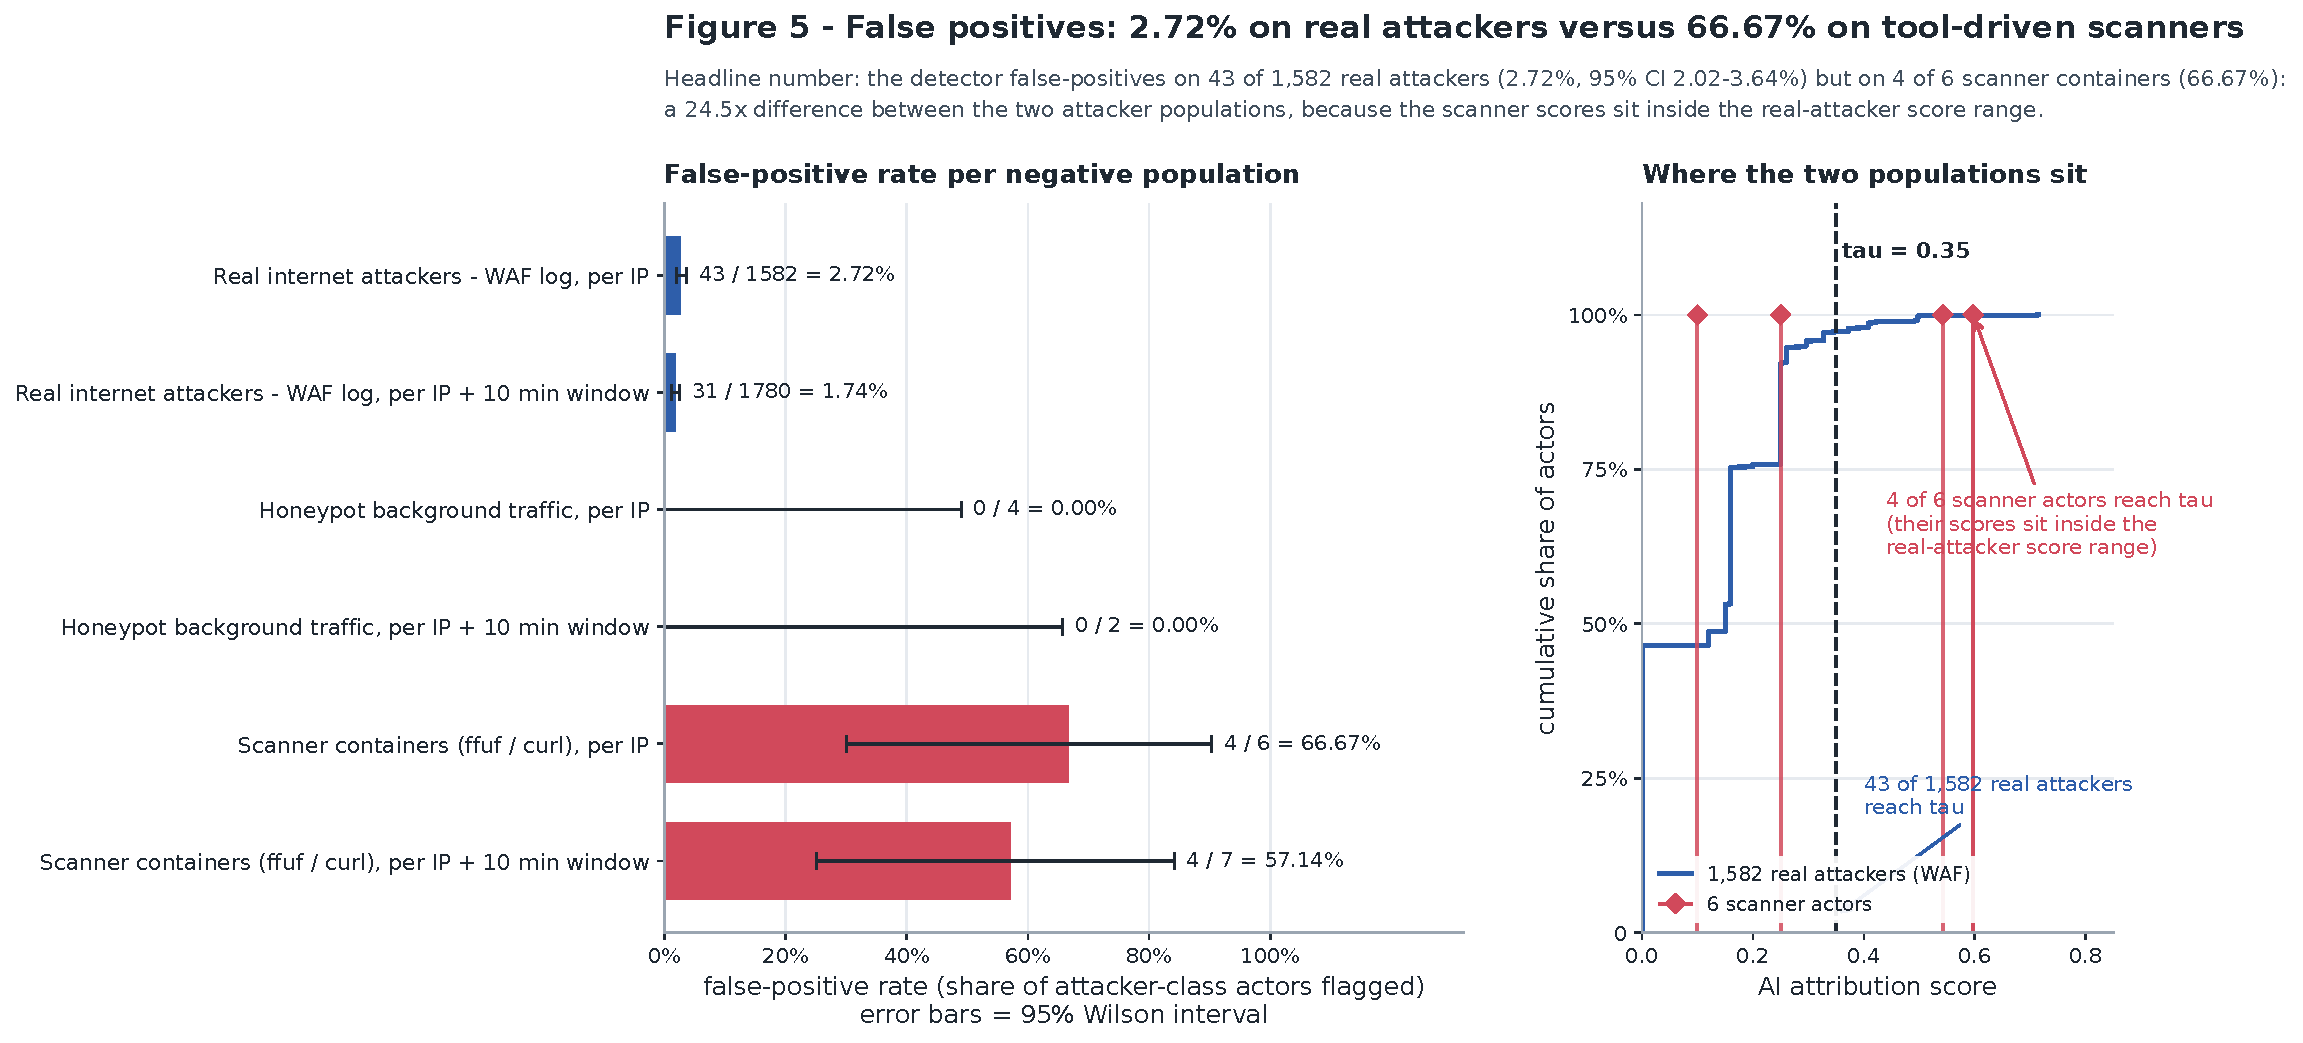
\includegraphics[trim=0 0 0 62.8bp,clip,width=0.88\textwidth]{figures/fig05_false_positive_breakdown.pdf}
\caption{False-positive rate of the six negative populations with 95\% Wilson intervals, next to
the cumulative score distribution of the two headline populations (1,582 WAF attackers and 6
scanner containers).
\textbf{Headline: 2.72\% false positives on the 1,582 real attackers (43/1,582) against
66.67\% on the six tool-driven scanner containers (4/6) --- a $24.5\times$ difference between
the two attacker populations; the honeypot population stays at 0\%.}}
\label{fig:08}
\end{figure}

The two numbers differ by more than an order of magnitude because the populations differ in
kind, not degree. The WAF-derived actors are predominantly browser-driven and interactive; the
scanner actors are enumeration tools. \ref{sec:boundary} develops this.

\subsection{Generalisation: leave-one-framework-out}
\label{sec:lofo}

Holding out each framework in turn and re-fitting the decision rule on the rest yields
detection in \textbf{9 of 10} folds. The failing fold is the framework with the smallest
capture (62 requests), which is below the volume the behavioural features require --- a
sampling limitation rather than a conceptual one.

Figure~\ref{fig:09} gives the per-fold recall and the one-sided lower bound as a function of
the framework count.

% source artwork: figures/fig07_leave_one_framework_out.pdf
\begin{figure}[t]
\centering
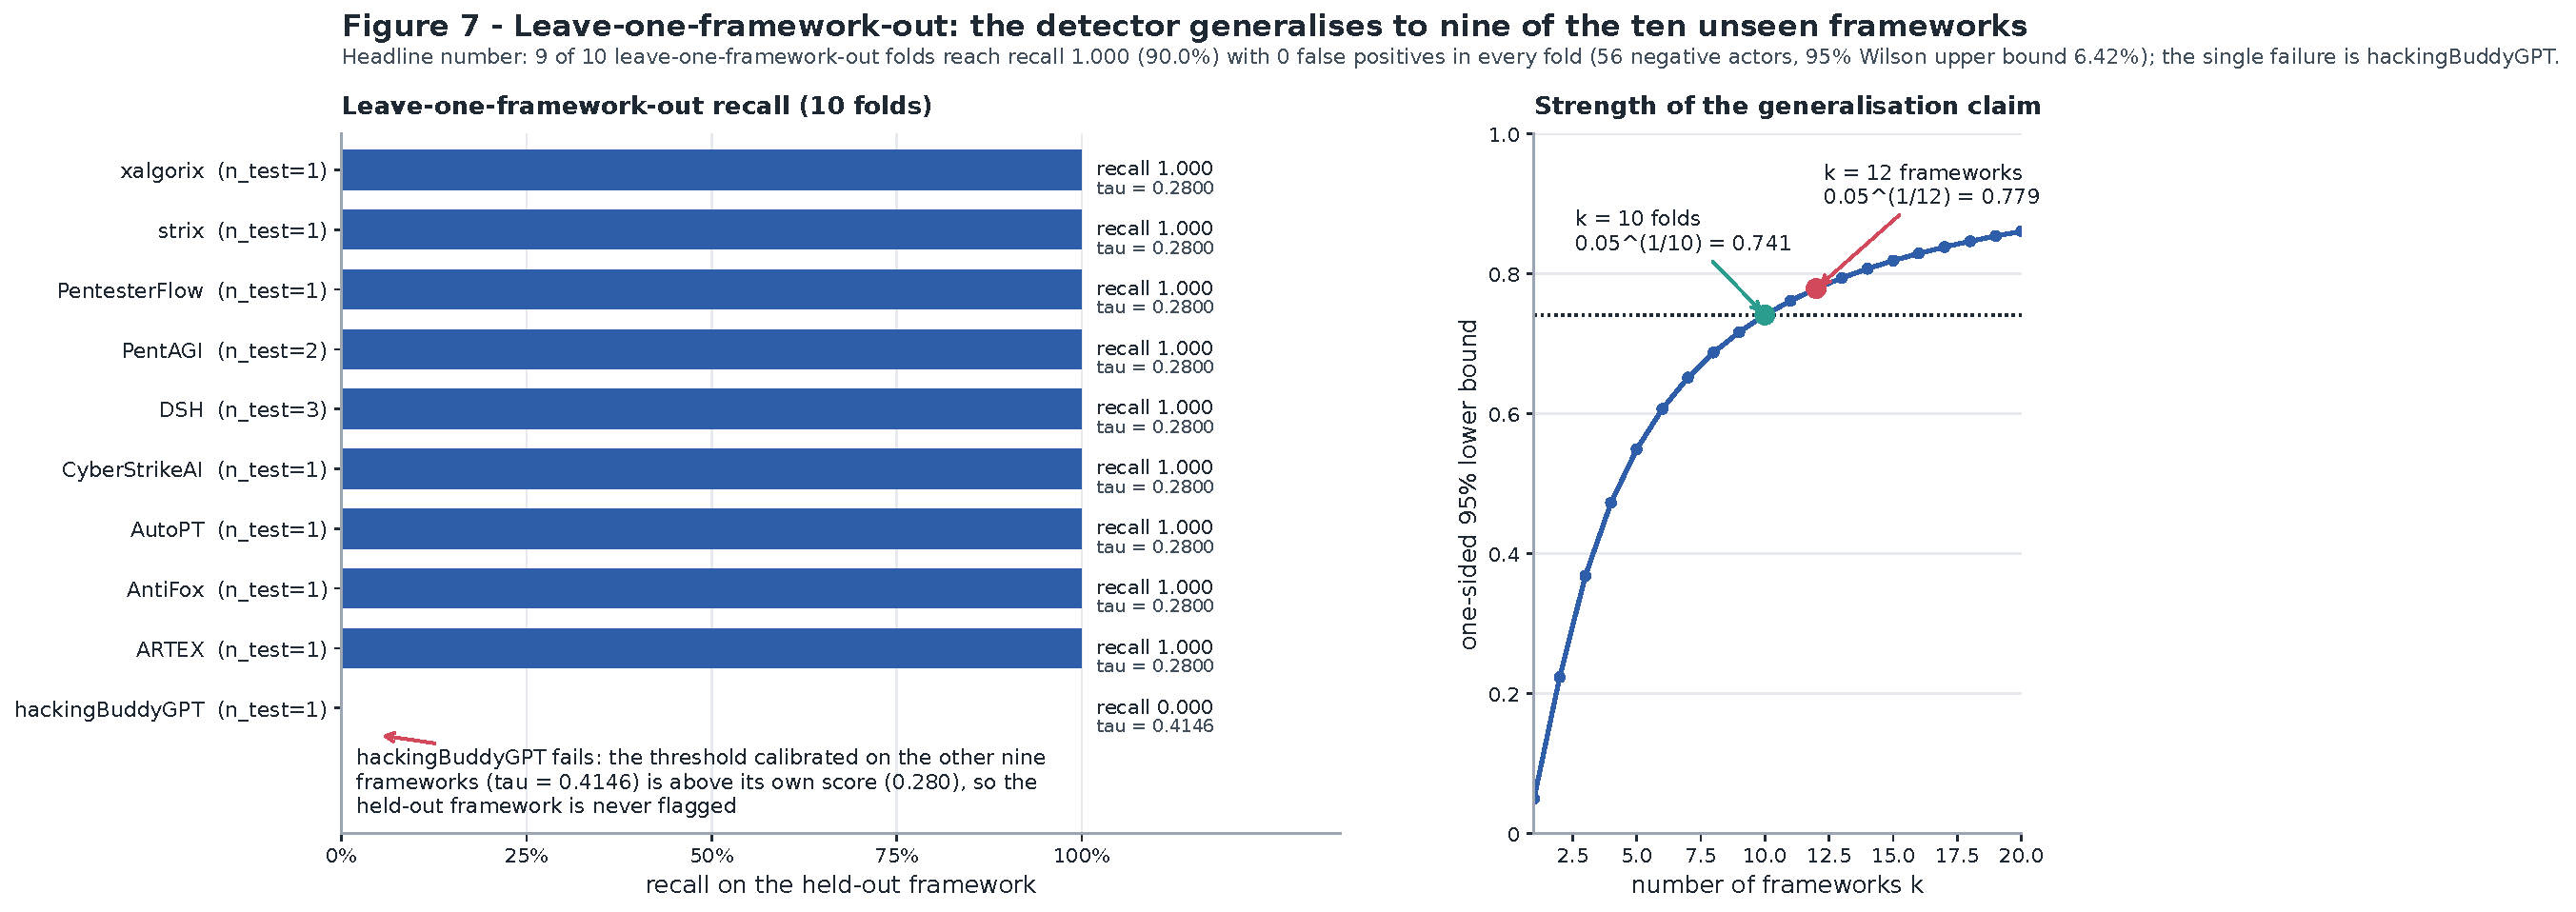
\includegraphics[trim=0 0 0 38.9bp,clip,width=0.88\textwidth]{figures/fig07_leave_one_framework_out.pdf}
\caption{Leave-one-framework-out recall over the 10 folds, with the threshold calibrated on the
other nine frameworks, and the one-sided 95\% lower bound $0.05^{1/k}$ of the generalisation
claim as a function of the framework count $k$.
\textbf{Headline: 9 of the 10 folds reach recall 1.000 (90.0\%) with 0 false positives in
every fold (56 negative actors, 95\% Wilson upper bound 6.42\%); the single failure is
hackingBuddyGPT, whose score (0.280) falls below the threshold calibrated on the other nine
frameworks ($\tau = 0.4146$).}}
\label{fig:09}
\end{figure}

\subsection{Family ablation}
\label{sec:ablation}

Removing one feature family at a time and measuring the recall ceiling:

\begin{table}[t]
\centering
\caption{Recall ceiling when one feature family is removed. F3 is the load-bearing family.}
\label{tab:ablation}
\begin{tabularx}{\textwidth}{@{}Y R{0.22\textwidth} R{0.22\textwidth}@{}}
\toprule
\textbf{Removed family} & \textbf{Recall ceiling} & \textbf{Change} \\
\midrule
none (base) & 0.933 & - \\
\textbf{F3} & \textbf{0.733} & \textbf{-0.200} \\
F6 & 0.867 & -0.067 \\
F4, F5, F7, F9, F10 & 0.933 & 0.000 \\
\bottomrule
\end{tabularx}
\end{table}

% source artwork: figures/fig06_feature_family_ablation.pdf
\begin{figure}[t]
\centering
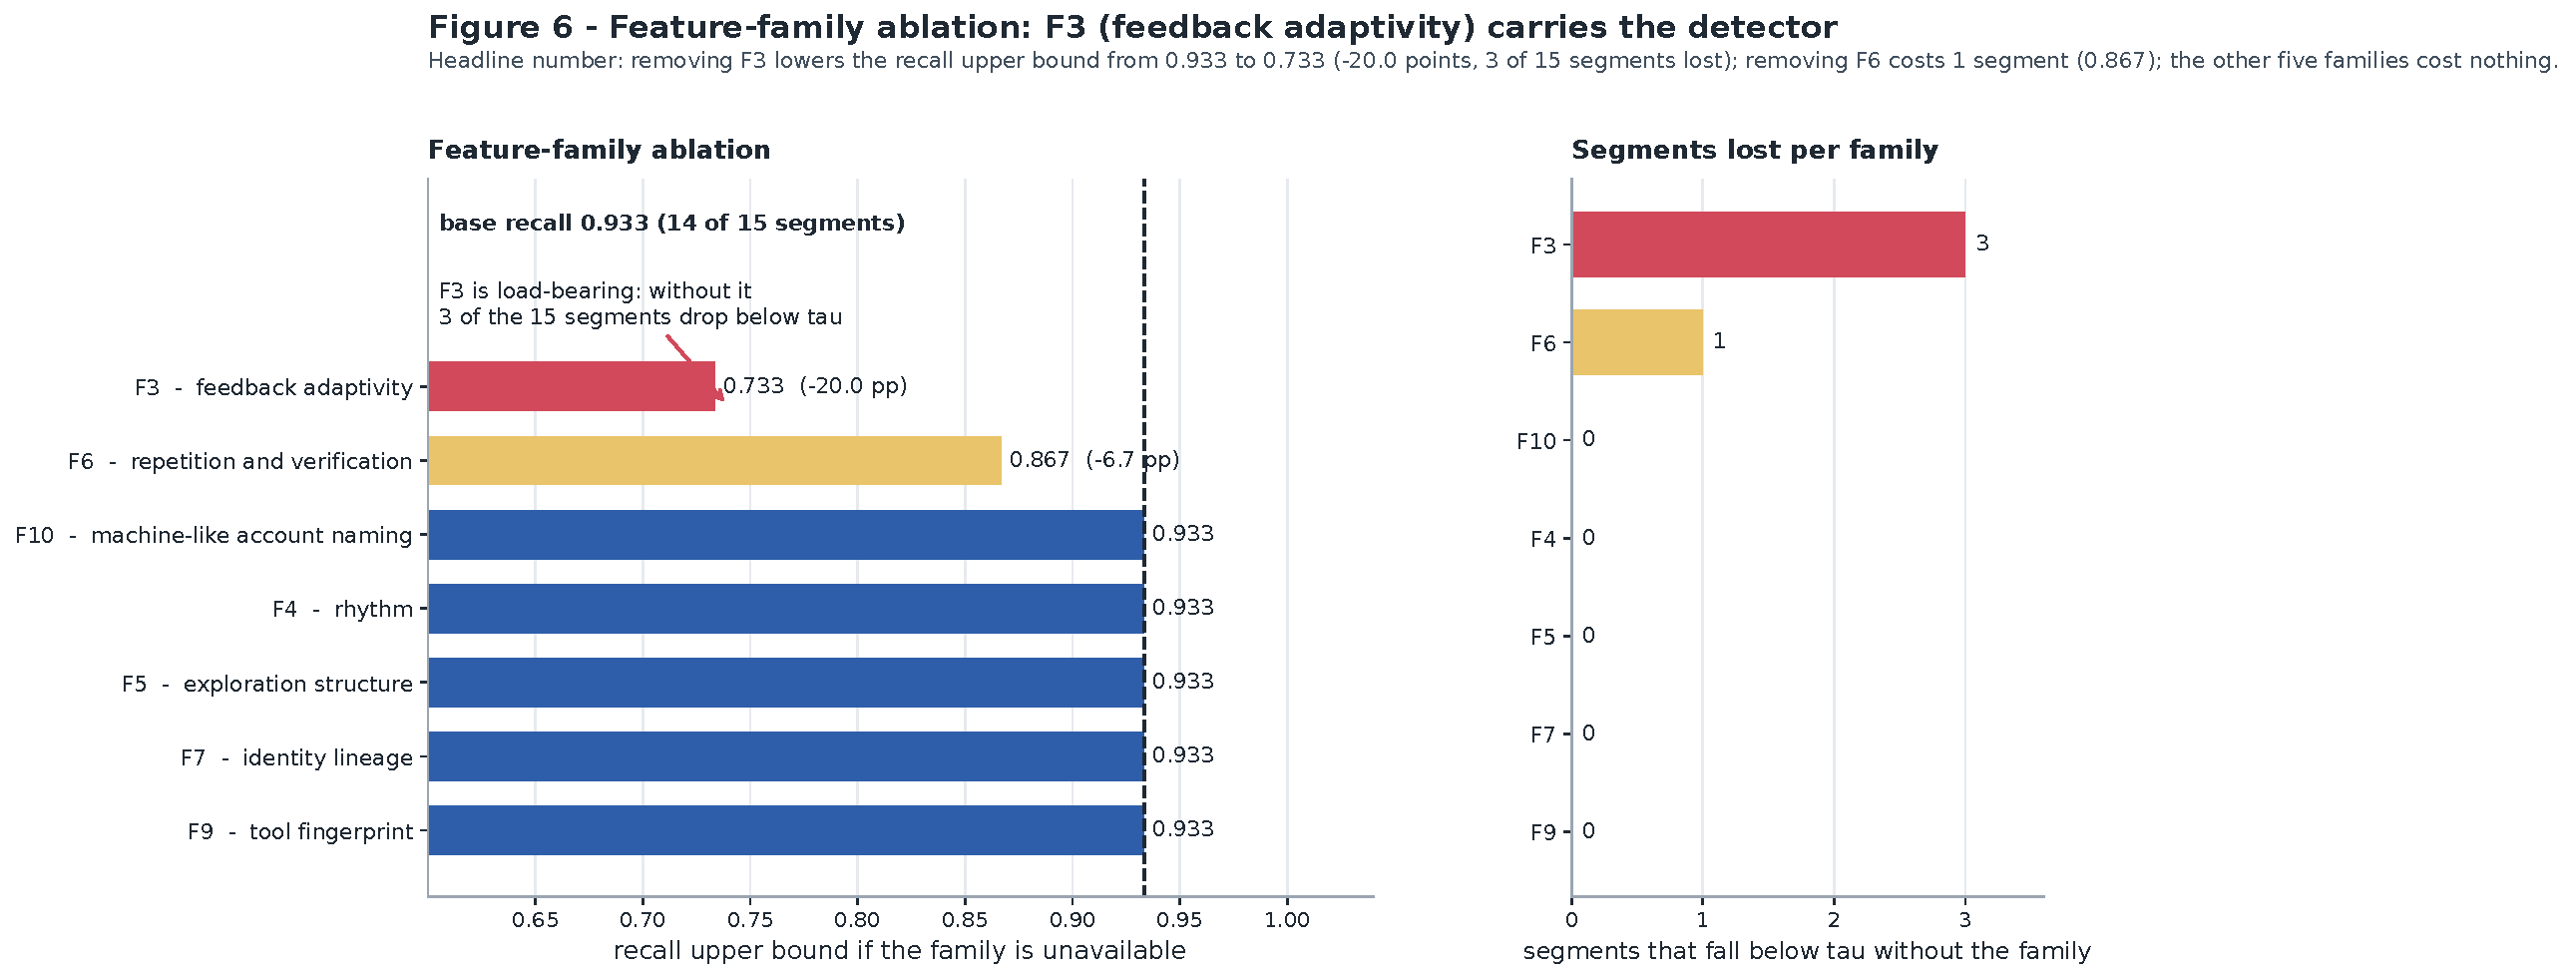
\includegraphics[trim=0 0 0 39.2bp,clip,width=0.88\textwidth]{figures/fig06_feature_family_ablation.pdf}
\caption{Feature-family ablation: the recall upper bound that remains when each feature family is
unavailable in the operator's logs, and the number of the 15 segments that fall below $\tau$
when the family is removed.
\textbf{Headline: the base recall upper bound is 0.933 (14 of 15 segments); removing F3
(feedback adaptivity) drops it to 0.733 (-20.0 points, 3 segments lost), removing F6
(repetition and verification) costs 1 segment (0.867), and the other five families cost
nothing.}}
\label{fig:10}
\end{figure}

Figure~\ref{fig:10} shows the same ablation as a per-segment breakdown.

F3 is the load-bearing family, exactly as the algebra predicted: it is the only family whose
three rules can jointly exceed the threshold, and it carries the post-error behaviour that
distinguishes an agent from a brute-force script.

% =====================================================================
\section{Discussion}
\label{sec:discussion}

\subsection{The attribution boundary}
\label{sec:boundary}

Three independent lines of evidence show that an AI agent which delegates its work to
general-purpose tooling is not distinguishable from a human using the same tooling.

\textbf{Evidence 1 --- an agent that calls sqlmap.} One audited framework, run live against
the evaluation target, spent its entire engagement inside a single tool invocation. Every
request the target observed carried \texttt{sqlmap/1.10.4}. The agent's own identity --- its
orchestration, its planning, its tool selection --- left no mark on the target at all.

\textbf{Evidence 2 --- scanner actors produce systematic false positives.} Six real enumeration
tools were run against the evaluation target in isolated containers and their traffic scored by
the behavioural detector. Four of the six were flagged at the operating threshold, and raising
the threshold did not reduce the count. The reason is structural: the features that separate an
agent from a human are features of \emph{adaptivity} --- switching endpoint family after an
error, revisiting an endpoint that returned success, rotating identities --- and a
well-written enumeration script exhibits the same behaviours when it is fed a wordlist.

\textbf{Evidence 3 --- a real agent degenerating into a tool.} A framework with an unusually
distinctive own signature was run in a low-intensity configuration. Its traffic was
characterised by 428 endpoint templates explored in 936 seconds, a 99\% 4xx ratio, a 1\% 2xx
rate and 442 requests per minute. The behavioural detector scored it 0.250 --- below threshold
--- and the reverse-evidence rule E15 classified it as a dictionary-driven enumerator. The
framework \emph{is} an AI agent, and the detector is right not to claim otherwise: at that
operating point the traffic carries no information that separates it from a human running the
same dictionary.

% source artwork: figures/fig10_ai_agent_vs_scanner_behaviour.pdf
\begin{figure}[t]
\centering
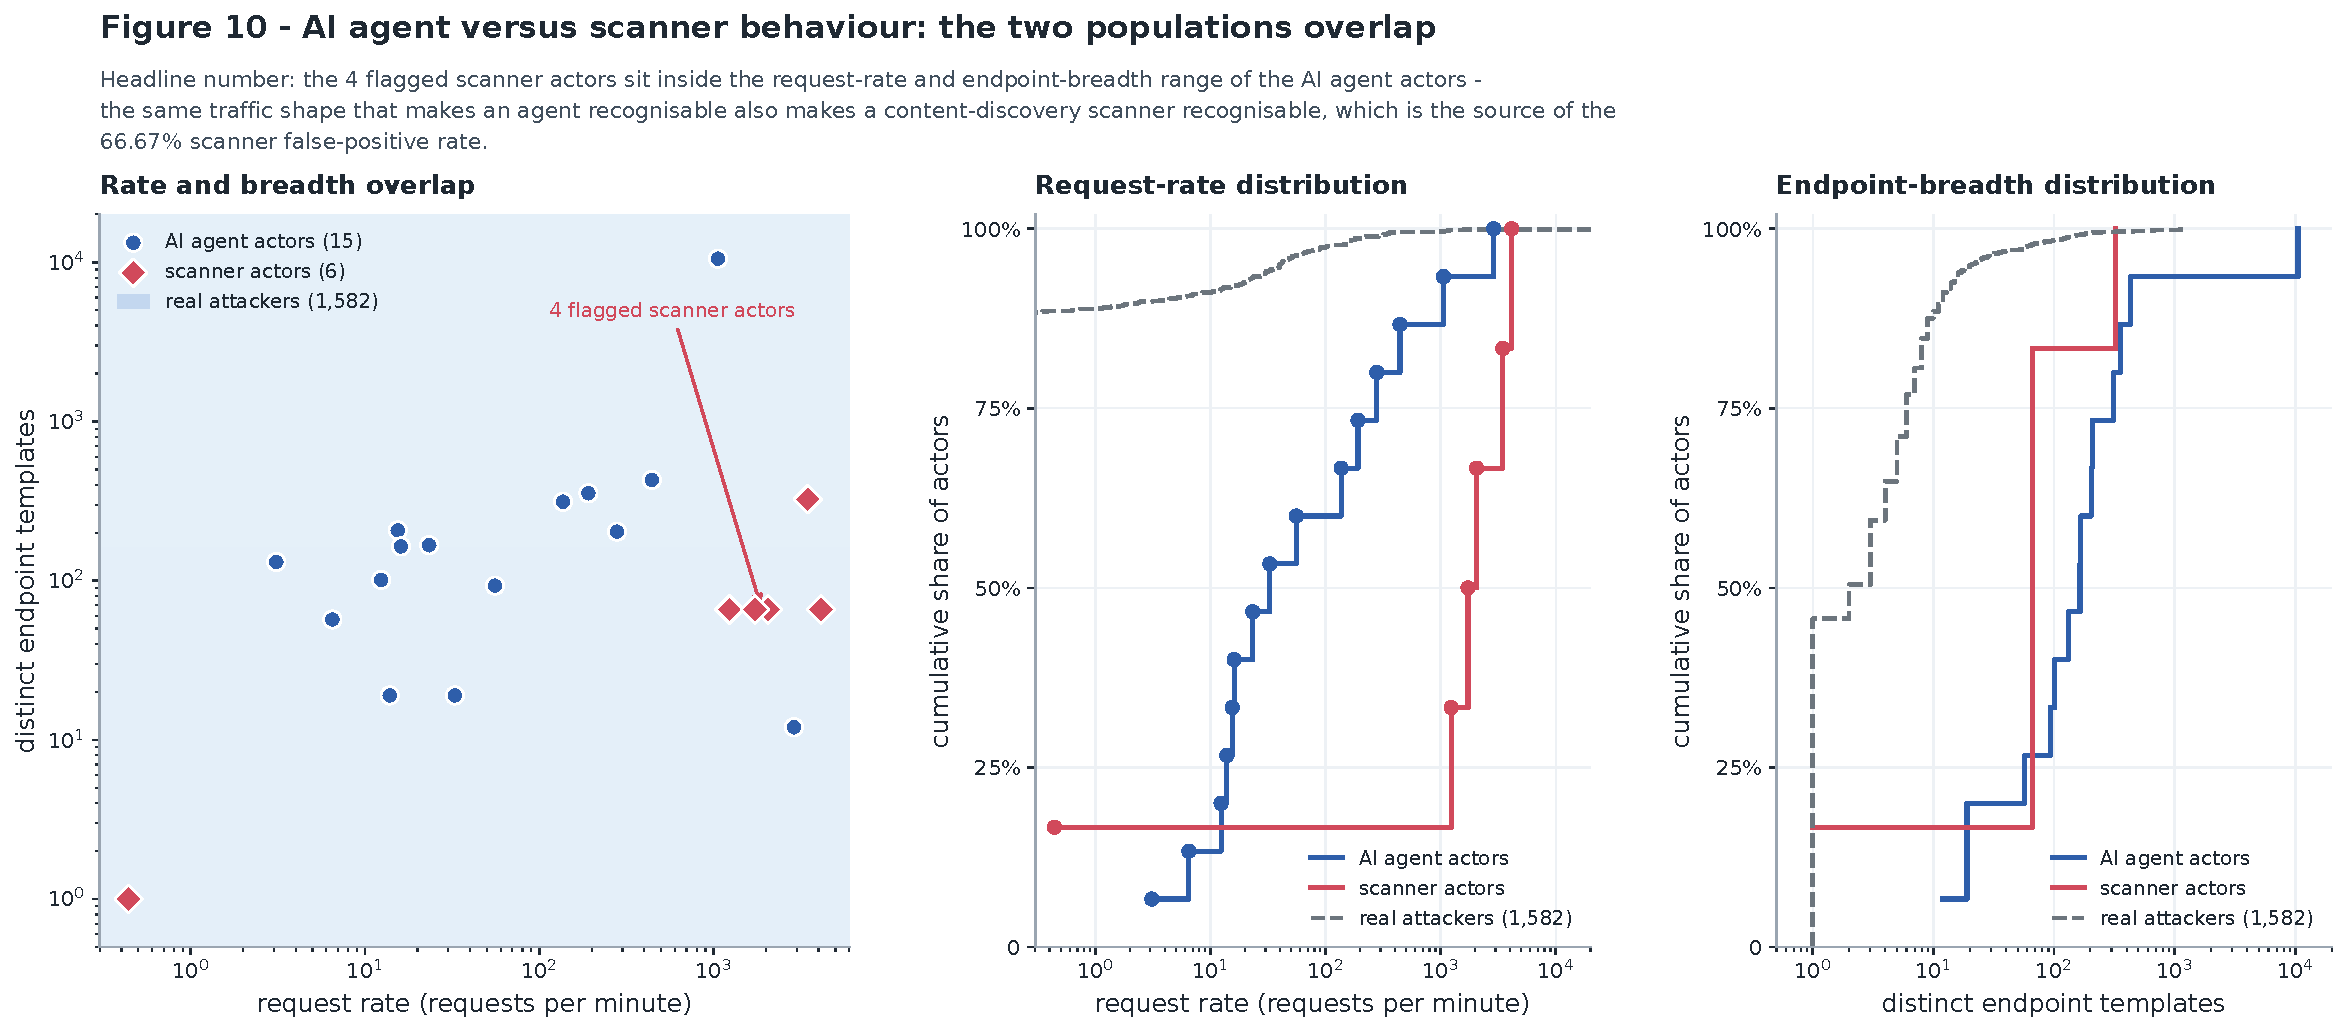
\includegraphics[trim=0 0 0 77.9bp,clip,width=0.88\textwidth]{figures/fig10_ai_agent_vs_scanner_behaviour.pdf}
\caption{AI agent versus scanner behaviour: the 15 AI agent actors, the 6 scanner containers and
the 1,582 real attackers in one plot of request rate against endpoint breadth, plus the
cumulative distributions of both variables.
\textbf{Headline: the four scanner actors that were flagged sit inside the request-rate and
endpoint-breadth range of the AI agent actors, which is the mechanical reason for the 66.67\%
scanner false-positive rate.}}
\label{fig:11}
\end{figure}

% source artwork: figures/fig12_feature_family_profile.pdf
\begin{figure}[t]
\centering
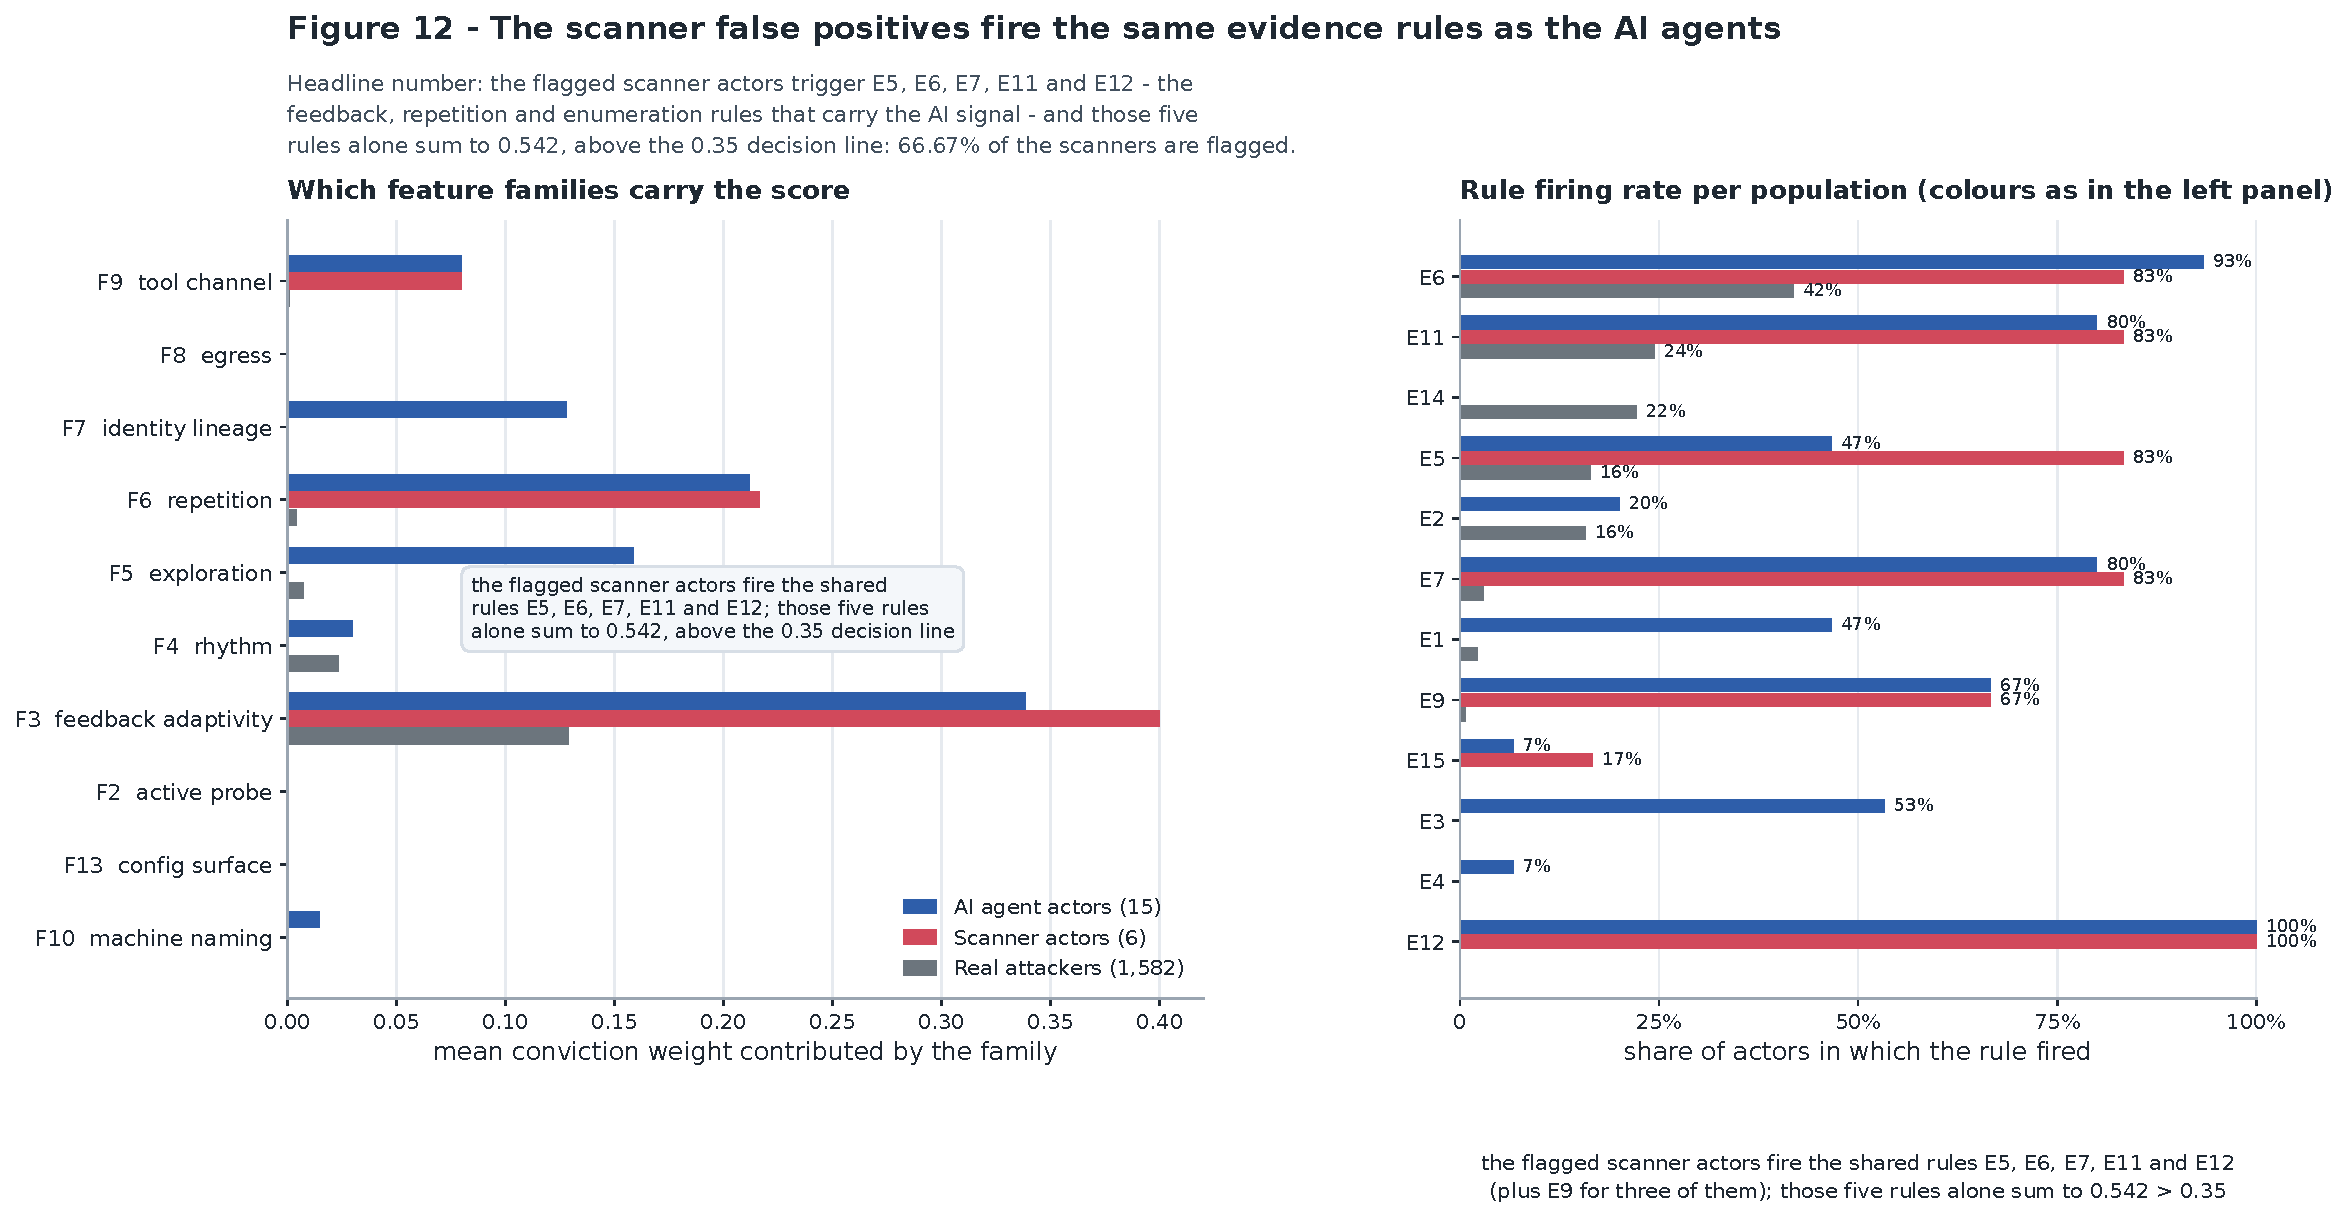
\includegraphics[trim=0 0 0 79.8bp,clip,width=0.88\textwidth]{figures/fig12_feature_family_profile.pdf}
\caption{Which feature families carry the decision: the mean conviction weight each feature
family contributes, for the AI agent actors, the scanner actors and the 1,582 real attackers,
and how often each evidence rule fires in the three populations.
\textbf{Headline: the flagged scanner actors fire the shared rules E5, E6, E7, E11 and E12
(plus E9 for three of them) and those five rules alone sum to 0.542, already above the 0.35
decision line --- which is why 66.67\% of the scanner actors are flagged.}}
\label{fig:12}
\end{figure}

Figure~\ref{fig:11} places the flagged scanner actors next to the AI agent actors and the
real attackers in the two dimensions the detector measures, and Figure~\ref{fig:12} shows
which feature families carry the decision in each of the three populations.

These three observations are the same phenomenon seen from three sides, and they bound what
passive HTTP inspection can achieve. When an agent is adaptive --- when its next request is
chosen in response to the previous response --- the behavioural signal exists and is
measurable. When the agent is running a fixed procedure, the signal is absent and no threshold
can manufacture it.

\subsection{What a defender can do}
\label{sec:defender}

\textbf{Deploy the T1 signatures for attribution, not for alerting on their own.} Their value
is precise: when one fires, the framework is identified. Their false-positive rate on real
traffic is zero over 10 million requests, and the combinatorial criterion keeps the alert
volume at one address per 81,000.

\textbf{Treat them as a complement to, not a replacement for, behavioural detection.} The
signatures answer which framework; the behavioural layer answers whether an agent was
involved. A deployment that expects signatures to answer both will conclude that AI agent
traffic is invisible whenever the agent delegates its work.

\textbf{Correlate egress traffic.} An agent must talk to an LLM provider. That traffic is
reliably attributable to an agent in a way that target-side traffic is not, and it is observable
on the same segment. This is the recommendation we make most strongly, and it is the one
control that survives the boundary described in \ref{sec:boundary}. We do not evaluate it here.

\textbf{Expect the signatures to decay.} \ref{sec:maintenance} discusses maintenance.

\subsection{Offensive risk of publishing this work}
\label{sec:egress}

Publishing signatures lowers the cost of evasion for a framework author who chooses to change
a User-Agent string. Publishing the behavioural thresholds lowers it further, because the
thresholds define exactly which behaviours are scored.

We accept that trade-off, for three reasons. The behavioural signals that matter are adaptive
behaviours --- switching family after an error, revisiting after success, rotating identities
--- and removing them costs the attacker the effectiveness that makes agentic attack worth
using; a genuinely adaptive agent cannot be made to look like a script without becoming one.
The signature half decays quickly regardless of publication, because frameworks change their
own markers as a matter of course. And the boundary finding in \ref{sec:boundary} is the most
useful thing in this paper for defenders, and it cannot be used to evade anything --- it
describes what is \emph{not} detectable.

The repository's \texttt{docs/THREAT\_MODEL.md} develops this analysis, including the
authors' view on which signatures should be withdrawn on request.

% =====================================================================
\section{Limitations}
\label{sec:limits}

\subsection{Statistical limitations}
\label{sec:statlimits}

The negative actor set contains 1,582 actors. That supports a false-positive rate estimate of
2.72\% with a 95\% interval of [2.02\%, 3.64\%], but it does \textbf{not} support a claim of
'below 1\%' --- the rule-of-three bound at this sample size is 0.19\%. Scanner-actor coverage is
smaller still: six actors, 999 requests, dominated by one tool (910 of 999 requests are from a
single enumeration tool), so the 66.67\% figure characterises that tool's behaviour rather than
a balanced multi-tool population.

The WAF-derived negative corpus contains no successful (2xx) responses --- a WAF records
requests it flags, not the traffic that passes --- so features that depend on success responses
are under-tested on that corpus.

The leave-one-framework-out evaluation covers ten frameworks, not sixty-five, because the other
fifty-five were never executed.

\subsection{Coverage limitations}
\label{sec:coverlimits}

Signatures reflect the audited revision of each framework and are invalidated by upstream
changes. Frameworks that were never executed contribute source-level signatures whose
target-side behaviour was inferred from code reading rather than observed. The framework count
of 65 is an audit count; the attribution count of 10 is a measurement count, and only the
second is evidence.

\subsection{Maintenance}
\label{sec:maintenance}

A signature set derived from source code decays as frameworks change. The maintenance model in
the repository's \texttt{CONTRIBUTING.md} asks framework authors to submit or confirm their
own signatures, on the grounds that they know their own markers better than a static audit can.
A submission or retraction request from an upstream maintainer is honoured.

% =====================================================================
\section{Reproducing the Results}
\label{sec:repro}

Every number in this paper is asserted by continuous integration against the shipped
artefacts. The dataset, the signature set and the evaluation code are in this repository.

\begin{lstlisting}
cd research
pip install -r requirements.txt

# score the published positive and negative captures
python pipeline/score_actor.py --input ../data/positive --out ../out/actor
python pipeline/score_actor.py --input ../data/negative --out ../out/actor-neg

# evaluation
python evaluation/evaluate_detection.py --actors ../out/actor --out ../out/metrics.json
python evaluation/false_positive_eval.py --features ../data/features --out ../out/fp.json
python evaluation/lofo.py --actors ../out/actor --out ../out/lofo.json
python evaluation/family_ablation.py --actors ../out/actor --out ../out/ablation.json
python evaluation/threshold_sweep.py --actors ../out/actor --neg ../data/features --out ../out/sweep.csv

# signature and headline validation (this is what CI runs)
python ci/check_signatures.py --rules ../signatures/rules.json --platform-dir ../signatures
python ci/check_signatures.py --rules ../signatures/agpl/rules-agpl.json --platform-dir ../signatures/agpl
python ci/selftest_rules.py --rules ../signatures/rules.json
python ci/check_headline_numbers.py
\end{lstlisting}

The reproducibility claim has a precise scope. Re-scoring the published captures reproduces the
recorded score exactly for 10 of the 15 positive captures; for the remaining five the published
file is the complete pseudonymised capture, whereas the recorded score was computed on the
agent-labelled subset of the original capture, so a full re-score is not directly comparable.
The numbers quoted in this paper are read from
\texttt{data/aggregate/framework\_detection.json}; the pipeline demonstrates that the
computation itself is reproducible.

The dataset card (\texttt{data/DATASET\_CARD.md}) records provenance, collection procedure,
licensing, intended use and the limitations of each corpus, including the pseudonymisation
scheme applied to the real-attacker actor set.

% =====================================================================
\section{Conclusion}
\label{sec:conclusion}

We audited 65 AI-pentest codebases (64 third-party frameworks plus one in-house
implementation), extracted 610 traffic signatures of which 272 are strong enough to deploy and
match zero rules across 10 million real requests and 142,705 real attack transactions, and
built an actor-level behavioural detector that reaches 86.7\% segment recall at a 2.72\%
false-positive rate on real attackers.

The more useful result is the boundary. Only 10 of the 65 audited codebases are attributable on
the target side; for the rest, the agent's identity does not reach the victim. Where the agent
delegates to general tooling, passive HTTP inspection cannot separate it from a human, and the
evidence for that is threefold and consistent. A defender who expects signatures alone to
answer the question will conclude that agentic traffic is invisible; the accurate statement is
narrower and more actionable: agentic traffic is visible when the agent is adaptive, and
invisible when it is not --- and the reliable signal in both cases is the agent's outbound
traffic to an LLM gateway, not its inbound traffic to the target.

All signatures, captured datasets and evaluation code needed to reproduce these numbers are
released with the paper at \url{https://github.com/Raven-Gt/ai-agent-attack-signatures}
\cite{aasrepo}.

% =====================================================================
\bibliographystyle{plain}
\bibliography{REFERENCES}

\noindent\textbf{Provenance note.} The 65 audited AI pentest frameworks are not cited as
bibliographic entries because we did not read a published paper for each of them; each is
cited by its upstream repository URL in the \texttt{NOTICE} file of the artefact repository
\cite{aasrepo}, with per-signature provenance (upstream repository, file path and line
number) recorded in the \texttt{framework} and \texttt{source} fields of
\texttt{signatures/rules.json}. The two public corpora used for signature validation are
cited above by their dataset and project URLs, and the artefact itself is cited by
repository URL.

\end{document}
